\documentclass[12pt,spanish,letter]{report}
\usepackage[T1]{fontenc}
\usepackage{lmodern}
\usepackage{amssymb,amsmath}
\usepackage{ifxetex,ifluatex}
\usepackage[left=2.6cm,top=3cm,right=2.6cm]{geometry}
\usepackage{fixltx2e} % provides \textsubscript
\usepackage[spanish,english]{babel}
\usepackage{anyfontsize}
\usepackage{mathptmx}

% \renewcommand{\familydefault}{\sfdefault}

% use microtype if available
\IfFileExists{microtype.sty}{\usepackage{microtype}}{}
\ifnum 0\ifxetex 1\fi\ifluatex 1\fi=0 % if pdftex
  \usepackage[utf8]{inputenc}
\else % if luatex or xelatex
  \usepackage{fontspec}
  \ifxetex
    \usepackage{xltxtra,xunicode}
  \fi
  \defaultfontfeatures{Mapping=tex-text,Scale=MatchLowercase}
  \newcommand{\euro}{€}
\fi
\usepackage{color}
\usepackage{fancyvrb}
\DefineShortVerb[commandchars=\\\{\}]{\|}
\DefineVerbatimEnvironment{Highlighting}{Verbatim}{commandchars=\\\{\}}
% Add ',fontsize=\small' for more characters per line
\newenvironment{Shaded}{}{}
\newcommand{\KeywordTok}[1]{\textcolor[rgb]{0.00,0.44,0.13}{\textbf{{#1}}}}
\newcommand{\DataTypeTok}[1]{\textcolor[rgb]{0.56,0.13,0.00}{{#1}}}
\newcommand{\DecValTok}[1]{\textcolor[rgb]{0.25,0.63,0.44}{{#1}}}
\newcommand{\BaseNTok}[1]{\textcolor[rgb]{0.25,0.63,0.44}{{#1}}}
\newcommand{\FloatTok}[1]{\textcolor[rgb]{0.25,0.63,0.44}{{#1}}}
\newcommand{\CharTok}[1]{\textcolor[rgb]{0.25,0.44,0.63}{{#1}}}
\newcommand{\StringTok}[1]{\textcolor[rgb]{0.25,0.44,0.63}{{#1}}}
\newcommand{\CommentTok}[1]{\textcolor[rgb]{0.38,0.63,0.69}{\textit{{#1}}}}
\newcommand{\OtherTok}[1]{\textcolor[rgb]{0.00,0.44,0.13}{{#1}}}
\newcommand{\AlertTok}[1]{\textcolor[rgb]{1.00,0.00,0.00}{\textbf{{#1}}}}
\newcommand{\FunctionTok}[1]{\textcolor[rgb]{0.02,0.16,0.49}{{#1}}}
\newcommand{\RegionMarkerTok}[1]{{#1}}
\newcommand{\ErrorTok}[1]{\textcolor[rgb]{1.00,0.00,0.00}{\textbf{{#1}}}}
\newcommand{\NormalTok}[1]{{#1}}
\usepackage{graphicx}
% We will generate all images so they have a width \maxwidth. This means
% that they will get their normal width if they fit onto the page, but
% are scaled down if they would overflow the margins.
\makeatletter
\def\maxwidth{\ifdim\Gin@nat@width>\linewidth\linewidth
\else\Gin@nat@width\fi}
\makeatother
\let\Oldincludegraphics\includegraphics
\renewcommand{\includegraphics}[1]{\Oldincludegraphics[width=\maxwidth]{#1}}
\ifxetex
  \usepackage[setpagesize=false, % page size defined by xetex
              unicode=false, % unicode breaks when used with xetex
              xetex]{hyperref}
\else
  \usepackage[unicode=true]{hyperref}
\fi
\hypersetup{breaklinks=true,
            bookmarks=true,
            pdfauthor={Borrador — Universidad Técnica Federico Santa María},
            pdftitle={Switch IDE: Desarrollo de un Entorno de Desarrollo Integrado con Constructor de Intefaces para Aplicaciones Web},
            colorlinks=true,
            urlcolor=blue,
            linkcolor=magenta,
            pdfborder={0 0 0}}
\setlength{\parindent}{0pt}
\setlength{\parskip}{6pt plus 2pt minus 1pt}
\setlength{\emergencystretch}{3em}  % prevent overfull lines


\setcounter{tocdepth}{5} %to make it appears in TOC
\setcounter{secnumdepth}{5} %to make it numbered

\linespread{1.1}

\renewcommand{\baselinestretch}{0.8}

\makeatletter
\renewenvironment{abstract}{%
  \if@twocolumn
    \section*{\abstractname}%
  \else
    \small
    \begin{center}%
      %\topskip0pt
    	  %\vspace*{\fill}
      {\bfseries \abstractname \vspace{-.5em}\vspace{\z@}}%
    	  %\vspace*{\fill}
    \end{center}%
    \quotation
  \fi}
  {\if@twocolumn\else\endquotation\fi}
\makeatother

% Title
\title{
\vspace{-3cm}
{\fontsize{18}{22} {\textbf{UNIVERSIDAD TÉCNICA FEDERICO SANTA MARÍA}}} \\
{\fontsize{16}{22} \textbf{DEPARTAMENTO DE INFORMÁTICA}} \\
{\fontsize{14}{17} \textbf{SANTIAGO, CHILE}} \\[25mm]
\Oldincludegraphics[scale=0.7]{figures/logo_utfsm.png} \\[1\baselineskip]
{\fontsize{20}{24} \textbf{"SWITCH IDE: CREACIÓN DE UN ENTORNO DE DESARROLLO INTEGRADO CON CONSTRUCTOR DE INTERFACES PARA APLICACIONES WEB"}} \\[1\baselineskip]
{\fontsize{14}{17} \textbf{IAN ALEXANDER MURRAY SCHLEGEL}} \\[\baselineskip]
{\fontsize{12}{17} \textbf{MEMORIA DE TITULACIÓN PARA OPTAR AL TÍTULO DE INGENIERO CIVIL INFORMÁTICO}} \\[\baselineskip]
{\fontsize{12}{17} \textbf{PROFESOR GUÍA: JOCELYN SIMMONDS}} \\
{\fontsize{12}{17} \textbf{PROFESOR CORREFERENTE: LIOUBOV DOMBROVSKAIA}} \\
}
\date{\fontsize{14}{17} {\textbf{NOVIEMBRE 2012}}}

% Begins the document!
\begin{document}

% Select spanish as default
\selectlanguage{spanish}

\maketitle

% Renew line separation
\renewcommand{\baselinestretch}{1}
\selectfont

% Roman pages for the first part of the thesis
\pagenumbering{Roman}

% Dedicatory
\begin{flushright}
\topskip0pt
\vspace*{\fill}

\textit{A los que creyeron en mí, a los que me apoyaron,\\a todos los que hicieron esto posible.}

\vspace*{\fill}
\end{flushright}

\clearpage
\newpage

% Abstract
\vspace*{\fill}
\vspace{-2.5cm}
\begin{abstract}

Hoy en día, para desarrollar aplicaciones web no existe una gran variedad de herramientas de código abierto o gratuitas que faciliten el prototipado de vistas en el proceso de desarrollo. Herramientas de escritorio como Visual Studio o Xcode, que facilitan en gran medida esta parte del desarrollo de aplicaciones para Windows y Mac respectivamente, no tienen una contraparte en el ambiente web que satisfaga los requerimientos antes dichos. En este trabajo se crea un Entorno Integrado de Desarrollo llamado Switch IDE que permite al desarrollador programar aplicaciones utilizando el framework Backbone de Javascript y un editor de interfaces en base a los widgets provistos por la librería Twitter Bootstrap. Finalmente se logra desarrollar la herramienta, basada en web, que según las pruebas preliminares permitiría ahorrar en promedio un 30\% del tiempo invertido en prototipar interfaces.
\\[\baselineskip]
\textbf{Palabras Clave:} aplicaciones web, interfaces, entornos de desarrollo, javascript

\end{abstract}


%\newpage
\selectlanguage{english}

\begin{abstract}

Nowadays, there isn't a great variety of open-source or free tools to develop web applications that make prototyping of views easier during the development process. Desktop tools like Visual Studio or Xcode, that make this part of the development process a whole lot easier in Windows and Mac respectively, don't have a counterpart in the web environment that satisfies the aforementioned requirements. In this research, an Integrated Development Environment called Switch IDE is created, that allows developers to program applications using the Backbone Javascript framework and an interface builder based on Twitter Boostrap's widget library. Finally, the tool is developed, and according to preliminary tests it might be able to save an average of 30\% of the time that is invested in interface prototyping.
\\[\baselineskip]
\textbf{Keywords:} web applications, interfaces, development environments, javascript

\end{abstract}
\vspace*{\fill}
\selectlanguage{spanish}

% Glossary

\chapter*{Glosario}

\begin{description}
	\item[API] ``Application Programming Interface''. Es una especificación que define una interfaz para que componentes de software puedan comunicarse entre ellos.
	\item[CSS] Hojas de estilo en cascada (``Cascading Style Sheets'' por sus siglas en inglés). Es un lenguaje que permite definir estilos para sitios web, como alineación de texto, negritas y cursivas, colores, etc.
	\item[HTML] Lenguaje de marcado de hipertexto (``Hypertext Markup Language'' por sus siglas en inglés). Es el lenguaje de etiquetas que se utiliza para crear páginas web, y es lo que los navegadores interpretan para mostrar los diferentes elementos en la página.
	\item[HTTP] ``Hypertext Transfer Protocol'', es el protocolo de transferencia de hipertexto utilizado más comúnmente por los navegadores para transferir páginas web.
	\item[IDE] Entorno Integrado de Desarrollo ( ``Integrated Development Environment'' en inglés). Es un programa que combina varias herramientas para desarrollo (como un editor de código y un editor de vistas).
	\item[Javascript] Es el lenguaje de programación utilizado por el navegador, y permite al desarrollador entregar dinamismo a los sitios que de lo contrario serían estáticos.
	\item[JSON] ``Javascript Object Notation''. Es una forma de representar datos (números, cadenas de texto, etc) en un formato liviano y simple, basado en la notación de objetos de Javascript.
	\item[ODM] ``Object Document Mapper''. Es una técnica de programación muy similar a ORM, en donde objetos y documentos almacenados en una base de datos son relacionados directamente, de manera que documentos en la base de datos son representados por objetos en el lenguaje de programación que se esté usando.
	\item[ORM] ``Object Relational Mapper''. Es una técnica de programación en donde objetos representan a registros en una base de datos relacional.
	\item[REST] ``Representational State Transfer'', es una técnica de arquitectura de servicios web en la que la interfaz se basa en representar objetos y acciones sobre ellos (como creación y eliminación, por ejemplo).
	\item[SQL] ``Structured Query Language''. Es un lenguaje de consultas utilizado en bases de datos relacionales.	
	\item[URL] ``Uniform Resource Locator'', es básicamente una dirección a internet, como por ejemplo \href{http://www.usm.cl}{http://www.usm.cl}.
\end{description}


% TOC
\hypersetup{linkcolor=black} \tableofcontents

\clearpage
\newpage

% Here we go
% GL&HF
\chapter{Introducción}

\pagenumbering{arabic}

En el contexto del desarrollo de aplicaciones web, existen dos grandes
``corrientes''. Por una parte, es posible desarrollar aplicaciones
completamente de lado de servidor. Esto significa que la aplicación
procesa todos los datos y genera todo lo que el usuario ve de forma
remota. Esta forma de desarrollar ha sido así durante muchos años y
sigue siendo una forma muy utilizada. Por otra parte, últimamente, con
el crecimiento de la comunidad de Javascript, y la constante mejora en
rendimiento de los navegadores modernos, se ha popularizado la idea de
llevar gran parte de la lógica de negocio y el procesamiento de datos al
cliente. Los navegadores modernos tienen cada vez más capacidad de
ejecutar procesos rápida y eficientemente, lo que tiene varias ventajas,
como por ejemplo, se aliviana la carga en los servidores, lo que permite
poder soportar a muchos más usuarios simultáneos, y las aplicaciones se
desempeñan mucho mejor, dado que se disminuye el retardo que hay en
transmitir datos entre el cliente y el servidor. Esto último es muy
importante al momento de crear aplicaciones web. Si bien toda página
web, sin importar su naturaleza, debería ser lo más rápida posible, las
aplicaciones web deben serlo por sobre todo. Al fin y al cabo, están
intentando imitar el comportamiento de aplicaciones nativas, pero a su
vez alivianando la carga a la que se somete un desarrollador al momento
de crear aplicaciones compatibles con una infinidad de dispositivos y
sistemas operativos distintos.

Desarrollar aplicaciones web versus desarrollar aplicaciones nativas
(que son ejecutables directamente en el computador, sin necesidad de un
navegador) tiene varias ventajas, siendo quizás la más importante que no
es necesario escribir el programa para diferentes plataformas, dado que
la mayoría de los navegadores modernos funcionan en una gran variedad de
dispositivos. Además, con el crecimiento del estándar HTML5 (que al
momento de escribir el presente documento aún se encuentra en proceso de
convertirse en un estándar final), es posible aprovechar muchas
características de los dispositivos (en algunos casos incluso es posible
usar los acelerómetros de los teléfonos móviles inteligentes). Es más,
muchos juegos han sido portados a la web, utilizando WebGL y tecnologías
similares.

Ahora bien, desarrollar aplicaciones web también tiene sus desventajas.
Es cosa de ver Xcode o Visual Studio, donde ambas herramientas son un
entorno completamente integrado para desarrollar aplicaciones. Desde
escribir código a crear formularios y diferentes tipos de vistas, ambas
herramientas (y otras similares) entregan una experiencia casi
inigualable al desarrollador. Al desarrollar aplicaciones y sitios web
en general, no es posible encontrar herramientas que se asemejen lo
suficiente a las mencionadas (y que sean de código abierto) como para
considerarse una alternativa viable. La mayoría de los entornos de
desarrollo para web permiten previsualizar lo que el desarrollador
codifica, pero no le permiten ahorrar tiempo al momento de realizar
tareas tan necesarias como codificar la interfaz de una aplicación.

Es este último aspecto el que se considera como un problema actualmente
en el mundo del desarrollo web. Si bien no es difícil codificar
interfaces de usuario al momento de crear aplicaciones web, es una tarea
que consume tiempo y para la cual sí existen herramientas muy buenas en
el mundo del desarrollo de aplicaciones nativas (como las ya mencionadas
Xcode o Visual Studio).

\section{Objetivos}

El objetivo primario de este trabajo es la creación de un entorno de
desarrollo integrado, al que se le llamará \textbf{Switch IDE}, que
permita el desarrollo de aplicaciones web facilitando la creación de
interfaces de manera similar a las herramientas descritas anteriormente.

Los objetivos secundarios de este trabajo serán:

\begin{itemize}
\item
  Permitir editar templates estilo Xcode o Visual Studio
\item
  Facilitar la estructuración de proyectos, evitando que el
  desarrollador programe todo en un solo archivo
\item
  Permitir ensamblar proyectos y probarlos directamente en Switch IDE
\item
  Liberar el código fuente de este trabajo bajo la licencia MIT {[}1{]}
\end{itemize}

\section{Estructura de este Trabajo}

El trabajo se estructurará como sigue:

\begin{itemize}
\item
  En el Capítulo \ref{section:state-of-the-art} se revisará primero el
  estado del arte, analizando las herramientas que actualmente intentan
  dar solución al problema identificado, además de frameworks y otro
  tipo de utilidades que mitigan de cierta forma el problema pero sin
  darle una completa solución.
\item
  Luego, en el Capítulo \ref{section:solution-proposal} se propondrá una
  solución al problema identificado.
\item
  Se construirá y documentará la creación de la solución planteada en el
  Capítulo \ref{section:construction}.
\item
  Se analizarán los resultados utilizando métricas que se describirán en
  el Capítulo \ref{sections:results}.
\item
  Finalmente, en el Capítulo \ref{section:conclusion} se presentarán
  conclusiones del trabajo junto con ideas para posible trabajo futuro.
\end{itemize}

\clearpage
\newpage

\chapter{Estado del Arte}

\label{section:state-of-the-art}

La metodología para el desarrollo de aplicaciones web está cambiando. Ha
pasado de estar enfocada casi completamente de desarrollar de lado de
servidor, a desarrollar parcial o totalmente de lado de cliente.
Frameworks como Backbone han revolucionado lo que se piensa sobre
desarrollar aplicaciones completamente usando Javascript, y la aparición
de muchísimos frameworks nuevos en este joven sub-mundo de aplicaciones
muestra claramente una tendencia hacia este ``paradigma''.

Ahora bien, el hecho de que periódicamente aparezcan nuevos frameworks
no es necesariamente bueno. Es fácil perderse, no se puede saber por
dónde empezar, y lo peor de todo, cada framework hace lo suyo de formas
diferentes, incluso utilizando paradigmas de desarrollo distintos (ya
sea MVC {[}2{]}, MVP {[}3{]} u otro de los que normalmente se utilizan).

En este capítulo, se revisarán las diferentes herramientas que existen
en el mundo del desarrollo de aplicaciones Javascript, además de
programas y utilidades que funcionan de manera similar a lo que se
quiere lograr con Switch IDE y que están actualmente en el mercado. Se
revisarán primero diferentes frameworks disponibles hoy en día,
analizando sus ventajas y desventajas, para luego mostrar herramientas
que facilitan el uso de frameworks.

\section{Frameworks Actuales}

Existe una variedad enorme de frameworks para desarrollo web de lado de
cliente, y, como se dijo anteriormente, día a día aparecen nuevos
competidores, lo que pasó de ser algo bueno a algo que aumenta las
barreras de entrada. El hecho de que haya tantas opciones para
desarrolladores (incluso experimentados) hace que elegir uno sea muy
difícil y que finalmente se opte por una solución posiblemente
incorrecta. Muchos frameworks tienen varios puntos fuertes, y no siempre
un framework es la mejor solución para un tipo determinado de problema.

Ahora bien, sí existen buenos frameworks y varios de ellos son
relativamente fáciles de entender y dominar. La mayoría de ellos llevan
buen tiempo en el mercado y por ende tienen una comunidad fuerte y
activa, junto con una base de código robusta.

\subsection{Backbone}

\label{sections:backbone}

\href{http://backbonejs.org}{Backbone} {[}4{]} es un framework simple,
extensible y liviano, lo que lo hace una muy buena opción para
desarrollar todo tipo de aplicaciones. Además, sus pocas dependencias de
otras librerías hacen que las aplicaciones desarrolladas con él sean más
livianas comparadas con otros frameworks.

El objetivo principal de Backbone es facilitar y dar estructura a
aplicaciones que se basan fuertemente en funcionar del lado del cliente
(es decir, en el navegador mismo). Normalmente, escribir aplicaciones de
este estilo es posible utilizando sólo Javascript y sin usar algún
framework, pero ello resulta tedioso, y lleva a aplicaciones difíciles
de mantener. Backbone (y la mayoría de los frameworks que se nombrarán
en este capítulo) intentan evitar esto último dándole una estructura a
las aplicaciones, separando vistas de controladores y modelos.

Es utilizado por una gran cantidad de sitios, tales como
\href{http://www.groupon.com/now}{Groupon Now!},
\href{http://trello.com}{Trello}, entre otros {[}5{]}. Las aplicaciones
nombradas no son proyectos pequeños y simples, sino que son aplicaciones
muy poderosas que se benfician muy bien de lo que Backbone provee.

Backbone es un framework de código abierto y por lo tanto completamente
gratuito.

\subsection{Cappuccino}

\href{http://cappuccino-project.org}{Cappuccino} {[}6{]} es un framework
de desarrollo web enfocado en llevar ``Cocoa'' de Apple a la web, aunque
no está en forma alguna afiliado con esta empresa. Abstrae completamente
el desarrollo web a un único lenguaje: Objective-J.

Las ventajas de este framework son varias. Al estar imitando frameworks
nativos de Apple, sigue varios estándares ya conocidos, y lo hace
bastante fácil de aprender para una persona con experiencia en
desarrollo iOS o Mac OS X. Además, todo se desarrolla con el mismo
lenguaje, y trae integrados varios widgets (botones, tablas, ventanas,
menús), lo que le permite al desarrollador enfocarse sólo en código y no
en el diseño (ver Figura \ref{figure:cappuccino}). A diferencia de
Backbone, en donde el desarrollador debe trabajar por un lado con el
código y por otro con el diseño y los estilos de las aplicaciones,
Cappuccino trae todo eso en un solo framework.

\begin{figure}[htbp]
\centering
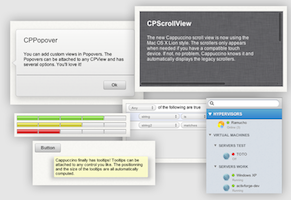
\includegraphics{figures/cappuccino-widgets.png}
\caption{Un ejemplo de los diferentes widgets que vienen incluidos en
Cappuccino. Puede apreciarse el diseño estilo OS X que trae.
\label{figure:cappuccino}}
\end{figure}

Una de las características interesantes de este framework, es la
capacidad de usar el constructor de interfaces de
\href{https://developer.apple.com/xcode/}{Xcode} {[}7{]} --- Interface
Builder --- para crear las interfaces. Eso sí, no todos los widgets que
están disponibles en Xcode están implementados en Cappuccino, y agregar
elementos inexistentes no siempre arroja errores fáciles de entender.
Además, desarrollar usando esta técnica, requiere instalar varios
componentes (entre ellos, Xcode, que no es una aplicación liviana) y se
necesita un computador Mac, dado que Xcode no funciona en otras
plataformas.

Además de lo anterior, tiene otras desventajas. Por un lado, es
necesario aprender un lenguaje nuevo (Objective-J). Por otro lado, hay
varios widgets esenciales que no están implementados, como por ejemplo,
controles de entrada de texto multilínea no está soportado actualmente
por el framework.

Cappuccino es un framework de código abierto y gratuito.

\subsection{Ext JS}

\href{http://www.sencha.com/products/extjs/}{Ext JS} {[}8{]} es un
framework con soporte para una gran variedad de widgets y es muy
poderoso. Una de las ventajas importantes de este framework, es que
existe una empresa detrás: \href{http://www.sencha.com/}{Sencha Inc}.
Esto hace del framework una herramienta continuamente soportada y en
constante desarrollo. Incluso, esta empresa ofrece soporte técnico
pagado para este framework.

Al llevar bastante tiempo circulando (desde el 2007 {[}9{]}), es un
framework con una gran cantidad de widgets y características disponibles
que lo hacen muy versátil. De la misma forma que Cappuccino, trae
integrados widgets como botones, tablas, ventanas, entre otros, pero con
la diferencia de que este framework sí está escrito en Javascript
directamente, por lo que no hace falta aprender un lenguaje nuevo.

Ahora, es un framework muy completo, por lo que su curva de aprendizaje
es más empinada comparándose con otras herramientas. Además, este
framework no es gratuito para desarrollo comercial. Si se desea
desarrollar una aplicación web y mantener el código propietario (es
decir, no liberarlo como código abierto), se deben cancelar (por lo
bajo) \$329 dólares americanos {[}10{]}.

\section{Herramientas Actuales}

Ahora que se han visto una variedad de frameworks disponibles para
desarrollar aplicaciones web, se procederá a analizar el mundo de las
herramientas para el desarrollo de éstas. El enfoque de esta sección es
analizar diferentes programas y servicios que se ofrecen, que son en
alguna forma similares a lo que se quiere lograr en el presente trabajo.

\subsection{Sencha Architect}

\href{http://www.sencha.com/products/architect}{Sencha Architect}
{[}11{]} es una herramienta que tiene varias similitudes con lo que se
quiere lograr en este trabajo. Es una herramienta de los mismos
creadores del framework Ext JS, es bastante poderosa, y permite
desarrollar aplicaciones web y móviles de manera visual.

\begin{figure}[htbp]
\centering
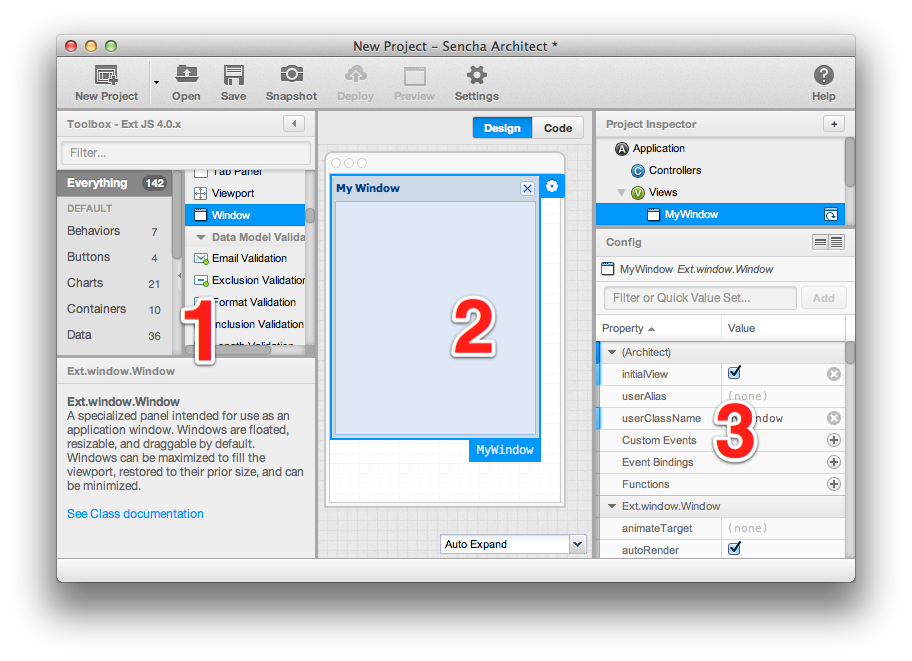
\includegraphics{figures/sencha-architect-big.png}
\caption{Sencha Architect: La ventana de trabajo
\label{figure:sencha-architect}}
\end{figure}

Sencha Architect es la herramienta que más se asemeja a un IDE para
desarrollo de aplicaciones nativas (como Xcode o Visual Studio). Posee
una barra lateral con componentes (ver Figura
\ref{figure:sencha-architect}, el número 1), un área central de trabajo
(número 2) y propiedades de los diferentes componentes que existan en el
área de trabajo (número 3).

Las ventajas de esta herramienta son claras: es posible crear las vistas
de las aplicaciones directamente, arrastrando componentes. De la misma
forma que herramientas para desarrollo nativo, esto ahorra tiempo al
momento de desarrollar.

En cuanto a las desventajas, el desarrollador está obligado a trabajar
con Ext JS como framework (que, como ya se dijo antes, es complejo de
dominar), y, por otro lado, el uso de este producto es pagado: cuesta
\$399 dólares americanos {[}12{]} al momento de escribir este documento.
Además, a ese valor hay que agregarle otros \$329 por la licencia de uso
de Ext JS {[}10{]}, si es que se quiere para uso comercial.

\subsection{Divshot}

\href{http://divshot.com/}{Divshot} {[}13{]} es una de las herramientas
que inspiró la presente memoria. Es una aplicación de prototipado rápido
basado en web. Fue creada en abril de 2012, por lo que es una
herramienta relativamente nueva.

Permite, utilizando Twitter Bootstrap {[}14{]}, crear prototipos de
sitios y aplicaciones web arrastrando componentes, de la misma forma que
IDEs como Xcode o Visual Studio (ver Figura \ref{figures:divshot}). En
la presente memoria, se quiere lograr un comportamiento muy parecido
para la creación de templates.

Entre las ventajas que presenta la herramienta, está la facilidad con la
que se pueden crear prototipos de vistas. Sólo arrastrando widgets, se
puede llegar a una vista en pocos minutos. Además, es posible
previsualizar los resultados fácilmente, e incluso exportar a
HTML\footnote{\textbf{Hypertext Markup Language:} es el lenguaje de
  etiquetas utilizado para las páginas web. Todas ellas están hechas con
  esto, más una combinación de otros lenguajes. {[}15{]}} con un sólo
click. Lo mejor de todo, es que el HTML generado está muy bien ordenado
y formateado.

Es una herramienta muy puntual y bien diseñada, pero sólo permite crear
vistas, no desarrollar. Además, es una herramienta de pago, y no es de
código abierto.

\begin{figure}[htbp]
\centering
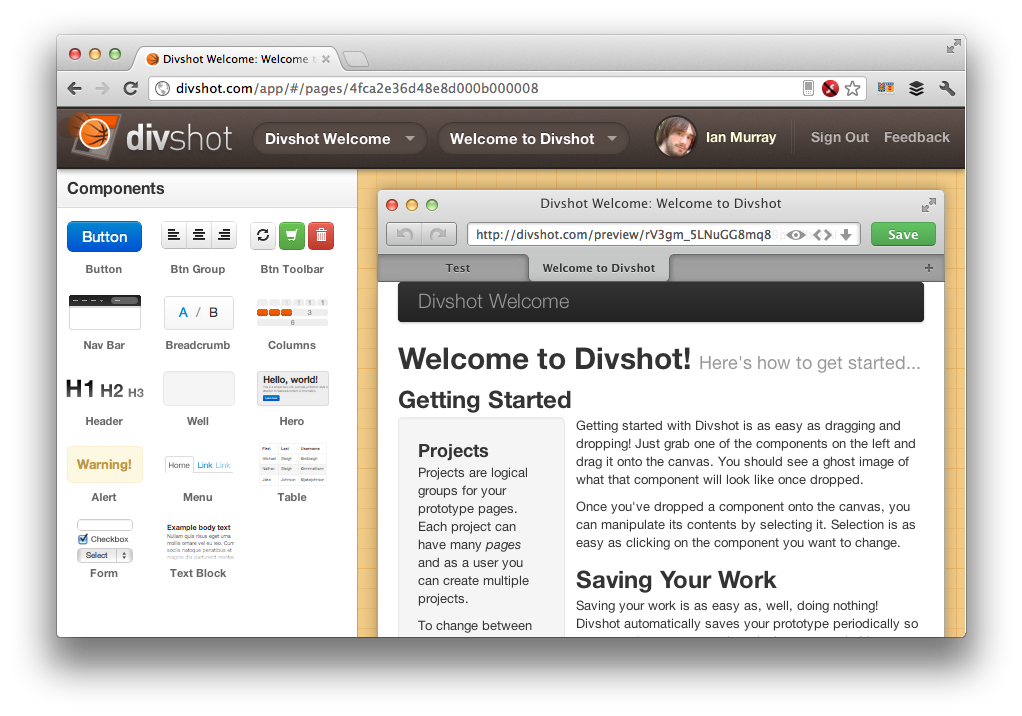
\includegraphics{figures/divshot-big.png}
\caption{La ventana principal de Divshot. Se pueden apreciar los
componentes en la barra lateral izquierda, con la vista a la derecha,
donde se arrojan los componentes. \label{figures:divshot}}
\end{figure}

\subsection{eXo Cloud IDE}

\href{http://cloud-ide.com}{eXo Cloud IDE} {[}16{]} es un entorno de
desarrollo integrado, en la nube. Tiene varias características que lo
hacen una buena opción al momento de querer colaborar o mantener el
código alojado en internet. Soporta una gran variedad de lenguajes
(entre ellos Java, Ruby y Python) y frameworks (como Ruby on Rails,
Spring o incluso Google App Engine).

Además de lo anterior, soporta plataformas como Heroku para subir
cambios a servidores directo desde el navegador, e incluso tiene soporte
para versionamiento con Git {[}17{]}.

Como cualquier IDE nativa estilo Xcode o Microsoft Visual Studio, tiene
un visor de los archivos actualmente abiertos (ver Figura
\ref{figure:exo-ide}, número 1) y el editor de código mismo (número 2).

\begin{figure}[htbp]
\centering
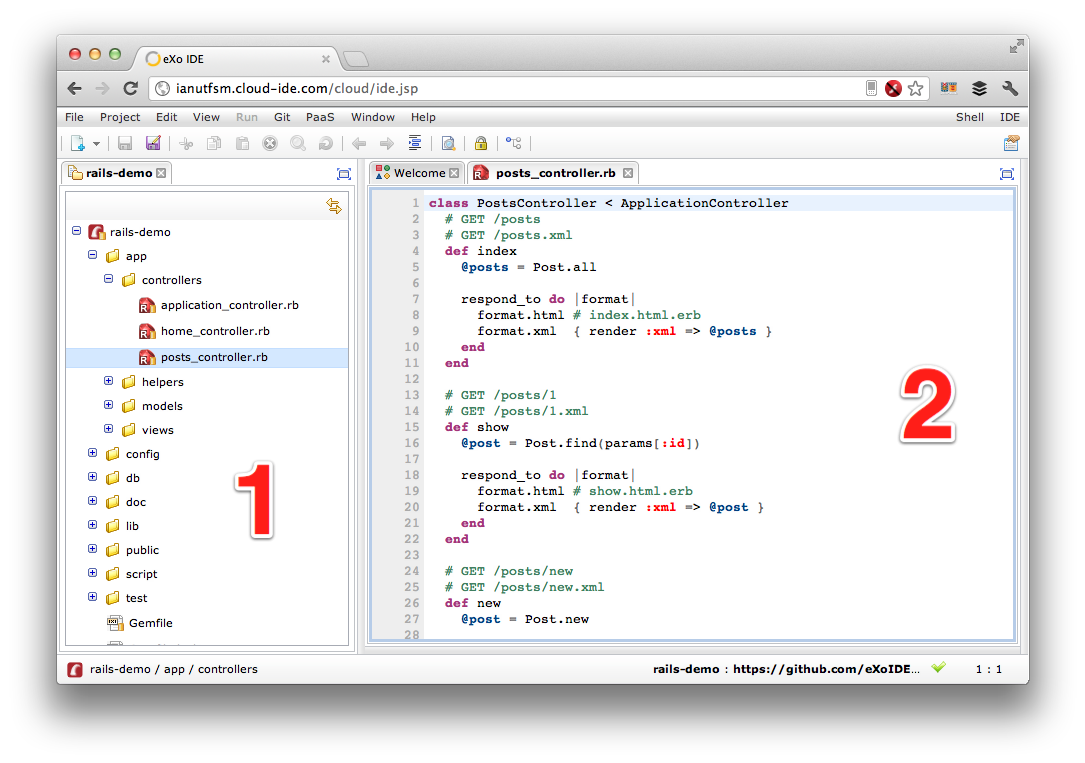
\includegraphics{figures/exo-ide-big.png}
\caption{eXo Cloud IDE: un entorno de desarrollo integrado, en la
nube\label{figure:exo-ide}}
\end{figure}

Las ventajas que provee esta herramienta son el no tener que depender de
un sólo equipo para desarrollar. Al mantener el código en la nube, sólo
es necesario conectarse al sitio web y empezar a trabajar. Por esto
último, tampoco es necesario instalar las diferentes herramientas
necesarias para desarrollar (como puede ser instalar Ruby o Python, que
a veces es engorroso).

Ahora bien, no permite crear templates de forma visual (que es lo que
uno espera de una herramienta integrada de este estilo). No permite
desarrollar aplicaciones de lado de cliente, sólo de lado de servidor, y
desarrollar aplicaciones con los frameworks que soporta por lo general
implica utilizar mucho el terminal de comandos para realizar pruebas, y
en un ambiente web, eso no es fácilmente replicable.

Es una herramienta de código cerrado pero gratuita.

\clearpage
\newpage

\chapter{Propuesta de Solución}

\label{section:solution-proposal}

Para solucionar el problema identificado, se propone crear Switch IDE,
una herramienta web (es decir, que sea accesible desde el navegador, y
no una aplicación nativa), que permita editar una aplicación web
completa en el mismo navegador, junto con permitir al desarrollador
crear templates de manera visual, en vez de utilizar sólo código.

El editor de templates deberá permitir al usuario crear las interfaces
que presentarían sus aplicaciones de manera visual, sin obligarlo a
escribir todo en código. Mediante el arrastre de diferentes widgets
prefabricados (como botones, formularios, ventanas modales, entre
otros), el usuario podrá generar templates en un tiempo menor y con
mayor facilidad que al hacerlo de la manera tradicional.

\section{Requisitos}

Principalmente, la herramienta será un Entorno de Desarrollo Integrado
compatible con Backbone (ver Sección \ref{sections:backbone}) y deberá:

\begin{itemize}
\item
  Permitir al usuario desarrollar aplicaciones utilizando el framework
  Backbone y Twitter Bootstrap. Se escogió Backbone por ser un framework
  simple y extensible, y por ser usado por varios sitios (ver Sección
  \ref{sections:backbone}). Se escogió Twitter Bootstrap {[}18{]} por su
  alta popularidad {[}19{]} y variedad de widgets.
\item
  Dar una estructura a las aplicaciones web, evitando que el
  desarrollador programe la aplicación completa en un sólo archivo
\item
  Facilitar la creación de vistas mediante un editor que permita
  arrastrar diferentes widgets a un ``canvas''
\item
  Permitir ensamblar y probar la aplicación de manera similar a cómo lo
  haría un programa nativo
\end{itemize}

Una herramienta con tales características no podrá funcionar sólo de
lado de cliente (exclusivamente en el navegador), dado que algunas
funciones tendrán que ser ejecutadas en el servidor, como por ejemplo la
compilación de los archivos Javascript o levantar una instancia de un
servidor para probar lo que el usuario esté desarrollando. Por esto, es
necesario implementar este proyecto en dos componentes distintas. Estas
dos componentes serán el backend y el backend, siendo el backend el
sistema que ``apoye'' al frontend, como se explica en la sección
siguiente, y el frontend la interfaz misma, lo que el desarrollador verá
de Switch IDE.

A continuación, se especificará qué roles cumplirán backend y frontend
en la herramienta propuesta, junto con sus requisitos específicos.

\subsection{Definición y Requisitos del Backend}

El backend será un servidor que permitirá al frontend realizar las
tareas que no le serán posibles por diferentes limitaciones. Por
ejemplo, los sitios web no pueden manipular archivos del sistema
operativo por motivos de seguridad, por lo que es imposible realizar
todo en el frontend. Por lo tanto, el backend cumplirá con las
siguientes tareas:

\begin{itemize}
\item
  Deberá generar los proyectos y sus estructuras (directorios y archivos
  base), junto con almacenarlos, dado que no es posible almacenarlos en
  el cliente
\item
  Manipular los archivos, es decir, crear, eliminar, renombrar y
  actualizar archivos y carpetas
\item
  Ensamblar los proyectos
\item
  Levantar servidores que permitan al desarrollador hacer pruebas
\end{itemize}

Es importante dejar claro que el usuario nunca deberá interactuar con el
backend directamente, será el frontend el que interactúe con éste y el
usuario no verá esta interacción.

\subsection{Definición y Requisitos del Frontend}

El frontend será el encargado presentarle al desarrollador todo lo que
necesite, como mostrar los archivos en un proyecto, mostrar un editor de
código o el editor de templates propuesto.

Específiamente, el frontend deberá permitir al desarrollador:

\begin{itemize}
\item
  Elegir entre diferentes proyectos existentes
\item
  Crear proyectos nuevos
\item
  Explorar los diferentes directorios de un proyecto abierto
\item
  Crear, renombrar y eliminar archivos y carpetas en un proyecto
\item
  Editar archivos, mediante un editor de código con resaltado de
  sintaxis
\item
  Editar visualmente los templates, listando diferentes widgets que el
  desarrollador podrá arrastrar a un ``canvas'' que se actualizará en
  tiempo real mostrando una vista previa del template
\item
  Ensamblar y probar el proyecto
\end{itemize}

\section{Elección de Herramientas}

En esta sección se discutirán las diferentes alternativas de
herramientas para desarrollar ambos el backend y el frontend, y qué
herramientas se escogieron finalmente.

\subsection{Elección de Herramientas para el Backend}

Existen varias alternativas en cuanto a la creación de un backend que
cumpla con los requisitos especificados anteriormente. Entre los
lenguajes más populares para el desarrollo de servicios web se
encuentran PHP, Java, Python y Ruby {[}20{]}. Para todos ellos existen
una variedad de frameworks para desarrollar servicios web (como
CodeIgniter {[}21{]}, Play {[}22{]}, Django {[}23{]} o Ruby on Rails
{[}24{]}, respectivamente). Además, todos permiten manipular archivos en
el servidor, que es uno de los requisitos especificados para el backend.

Si bien el autor tiene conocimiento de todos los lenguajes mencionados,
está más familiarizado con el último (Ruby). Además, para este lenguaje
existen diferentes librerías que permitirían agregar funcionalidad extra
en otra oportunidad (como Grit, una librería para manipular repositorios
Git desde Ruby {[}25{]}).

Lo que se quiere desarrollar en el lado del backend es básicamente una
API (Application Programming Interface) que el frontend utilizará parar
funcionar correctamente. Existen varias formas de programar APIs en
Ruby, y las más populares son Ruby on Rails y Sinatra {[}26{]}.

Ruby on Rails es un framework extremadamente completo, y el más popular
entre programadores de Ruby. Facilita una gran cantidad de tareas que
son tediosas en otros frameworks, lo que la hace una herramienta ideal
para todo tipo de proyectos web. Sin embargo, al ser una herramienta tan
completa, agrega bastante overhead. Además, es una herramienta ideal
para crear proyectos grandes y complejos, y dado que el backend de el
presente trabajo no requerirá tanta complejidad, se convierte en una
alternativa no tan ideal para este trabajo.

Sinatra es una versión simplificada de Ruby on Rails. Es un framework
más simple y liviano, por lo que inicia más rápido y, en general, se
desempeña mejor que su contraparte. Tiene la desventaja de no poseer
tantas facilidades para desarrollar sitios complejos, pero dado que el
backend de este proyecto no requerirá tanto trabajo, se considera como
la mejor opción y se utilizará para desarrollar el backend.

El backend requerirá una base de datos para poder guardar información de
los usuarios y proyectos. Se consideraron dos alternativas: MySQL
{[}27{]} y MongoDB {[}28{]}. La primera es una base de datos
convencional y la más popular {[}29{]}. La segunda es una base de datos
no relacional. Permite almacenar ``documentos'', o, más específicamente,
objetos del estilo JSON {[}30{]}. Además, no acepta consultas SQL, si no
que las consultas se realizan utilizando métodos directamente en la base
de datos.

Las ventajas que tiene MongoDB sobre MySQL son varias, entre algunas:
configurar escalamiento horizontal es relativamente sencillo, y permite
almacenar archivos en él usando una tecnología llamada GridFS {[}31{]}.

En términos de uso, existen librerías en Ruby para interactuar con ambas
bases de datos. Para MySQL, es posible usar ActiveRecord {[}32{]}, un
ORM muy popular y muy poderoso que
permite hacer consultas a la base de datos sin utilizar SQL. Para
MongoDB, existe Mongoid {[}33{]}, un ODM que provee una
interfaz muy similar a ActiveRecord.

Las ventajas que posee MongoDB por sobre MySQL hacen de ella una mejor
opción, dado que de ser necesario, podría migrarse el almacenamiento de
archivos a la base de datos y configurar escalamiento
horizontal\footnote{Escalamiento Horizontal en MongoDB: permite
  distribuir los datos almacenados en la base de datos en diferentes
  instancias de MongoDB, efectivamente distribuyendo la carga a la base
  de datos entre diferentes máquinas.
  http://docs.mongodb.org/manual/core/sharding/\#sharding-overview\ref{referencias}}
más fácilmente que de utilizar MySQL. De todas formas, en caso de querer
cambiar el sistema de base de datos, no se requerirían muchos cambios
dadas las similitudes de las librerías que existen.

Por último, como ya se describió antes, el backend deberá encargarse de
crear y estructurar proyectos. Para esto, existe una utilidad llamada
Brunch {[}34{]}. Brunch es un ensamblador de aplicaciones (``application
assembler'' en inglés). Básicamente, basándose en una plantilla,
organiza aplicaciones en carpetas. Soporta diferentes frameworks y
lenguajes, desde Backbone a Knockout {[}35{]}, usando Javascript o
Coffeescript {[}36{]}. Además de permitir estructurar los proyectos, los
ensambla, es decir, toma todos los archivos y los junta en uno sólo de
manera de optimizar la aplicación cuando esté en producción. Utilizar
esta herramienta en el backend permitirá crear y mantener proyectos
mucho más fácilmente que si se hiciera de forma manual

\subsection{Elección de Herramientas para el Frontend}

Para el desarrollo de aplicaciones de lado de cliente existen varios
frameworks, entre ellos Backbone, Knockout y Ember {[}37{]}. Todos ellos
poseen sus ventajas y desventajas. Por ejemplo, Knockout provee bindings
entre los modelos y las interfaces, mientras que Backbone es un
framework enfocado en simplicidad y rapidez. De hecho, en {[}38{]} se
menciona que incluyendo comentarios, posee tan sólo 1400 líneas de
código.

Considerando que la solución propuesta permitirá al usuario desarrollar
aplicaciones utilizando Backbone, además de que este framework se enfoca
en simplicidad, se prefirió frente a las otras alternativas

En cuanto a la interfaz, se prefirió utilizar Twitter Bootstrap, dado
que se encuentra en los requisitos permitir prototipar templates usando
este framework. Es un conjunto de widgets y un framework de prototipado
en HTML (es decir, no sólo trae widgets, sino que permite organizarlos y
estructurarlos), es extremadamente popular (es el repositorio más
popular en GitHub {[}19{]}) y es muy completo, proveyendo de todo tipo
de widgets que podrían encontrarse en herramientas como Visual Studio o
Xcode.

Ahora, Backbone es un framework que no da una estructura a las
aplicaciones que se desarrollan con él. A diferencia de, por ejemplo,
Ruby on Rails, la tarea de estructurar la aplicación en carpetas o
módulos depende completamente del desarrollador. En este punto se
asemeja mucho más a Sinatra que a Ruby on Rails. Esto podría
considerarse una desventaja, dado que sistemas complejos tienden a
crecer y desordenarse bastante si no se aplica una estructura desde un
principio.

Por las razones antes descritas, es que se decidió utilizar Brunch. Esta
herramienta ya se describió anteriormente, y permitirá facilitar el
desarrollo del frontend. Es más, incluye un servidor web de desarrollo,
que detecta cambios en los archivos y reensambla todo el sitio de manera
de poder hacer pruebas.

En lo que respecta la decisión de lenguaje de programación, no hay
muchas alternativas. Es posible desarrollar la solución usando
Javascript o Coffeescript. Existen otras alternativas (como TypeScript
de Microsoft {[}39{]}), pero al momento de escribir este documento no se
encuentran en etapas estables de desarrollo ni madurez. Javascript es un
lenguaje poderoso pero a la vez de relativo bajo nivel. Ciertas cosas
son un tanto tediosas de programar, como recorrer arreglos por ejemplo.
En cambio, Coffeescript, un lenguaje de programación escrito por Jeremy
Ashkenas que apareció en el 2009 {[}36{]} y que compila a Javascript,
hace que desarrollar en esta plataforma sea mucho más cómodo y simple,
sin perder desempeño ni funcionalidad (pues compila directamente a
Javascript). Además, Javascript es un lenguaje orientado a objetos en
base a prototipos, a diferencia de otros lenguajes (como Ruby o Java)
que son basados en la definición de clases. Coffeescript abstrae el
prototipado de objetos en Javascript permitiendo escribir clases de una
forma más simplificada.

A modo de ejemplo (y uno muy sencillo), podemos ver que para crear una
clase que permita extraer la primera palabra de una cadena de texto en
Javascript quedaría como sigue:

\begin{Shaded}
\begin{Highlighting}[]
\KeywordTok{var} \NormalTok{TextUtilities;}
\NormalTok{TextUtilities = (}\KeywordTok{function}\NormalTok{() \{}
  \KeywordTok{function} \NormalTok{TextUtilities() \{\}}
  \KeywordTok{TextUtilities.prototype}\NormalTok{.}\FunctionTok{initialize} \NormalTok{= }\KeywordTok{function}\NormalTok{(string) \{}
    \KeywordTok{return} \KeywordTok{this}\NormalTok{.}\FunctionTok{string} \NormalTok{= string;}
  \NormalTok{\};}
  \KeywordTok{TextUtilities.prototype}\NormalTok{.}\FunctionTok{firstWord} \NormalTok{= }\KeywordTok{function}\NormalTok{() \{}
    \KeywordTok{return} \KeywordTok{this}\NormalTok{.}\FunctionTok{string}\NormalTok{.}\FunctionTok{split}\NormalTok{(}\StringTok{" "}\NormalTok{)[}\DecValTok{0}\NormalTok{];}
  \NormalTok{\};}
  \KeywordTok{return} \NormalTok{TextUtilities;}
\NormalTok{\})();}
\end{Highlighting}
\end{Shaded}

En cambio, con CoffeeScript, lo mismo se resume a lo siguiente:

\begin{Shaded}
\begin{Highlighting}[]
\KeywordTok{class} \DataTypeTok{TextUtilities}
  \NormalTok{initialize}\KeywordTok{:} \FunctionTok{(string) ->} \DataTypeTok{@string} \KeywordTok{=} \NormalTok{string}
  \NormalTok{firstWord}\KeywordTok{:} \FunctionTok{->} \DataTypeTok{@string}\KeywordTok{.}\NormalTok{split}\KeywordTok{(}\StringTok{" "}\KeywordTok{)[}\DecValTok{0}\KeywordTok{]}
\end{Highlighting}
\end{Shaded}

\clearpage
\newpage

\chapter{Construcción de la Solución}

\label{section:construction}

Este capítulo tiene por objetivo detallar todo el proceso del diseño y
desarrollo de la solución propuesta anteriormente. Se dividirá en los
siguientes subcapítulos:

\begin{itemize}
\item
  Introducción a Backbone: en la Sección \ref{section:object-definition}
  se introducirán algunos de los conceptos necesarios para entender cómo
  funciona Backbone.
\item
  Diseño de la solución: en la Sección \ref{section:solution-design} se
  explicará cómo ambas componentes (frontend y backend) interactuarán
  entre sí. Además, se describirá cómo funcionarán ambas partes en
  términos de manipulación de archivos y el proyecto completo. Por
  último, se explicará cómo se diseñó el componente principal de la
  solución (el editor de interfaces).
\item
  Construcción de la base: el desarrollo de la solución se dividió en
  dos etapas. Como se verá en la Sección \ref{section:first-stage},
  primero se desarrolló lo que se consideró una ``base'' del programa.
  Esta etapa contempló el desarrollo de gran parte del backend y, en el
  frontend, una herramienta que permitiera crear proyectos nuevos,
  crear, editar y eliminar archivos, compilar y correr el proyecto.
\item
  Construcción del editor de interfaces: en la Sección
  \ref{section:interface-editor} se verá la segunda parte del
  desarrollo, que se enfocó en desarrollar y perfeccionar el editor de
  interfaces. Dado que este componente es la parte más importante de la
  solución, se decidió dedicar una etapa completa a él.
\end{itemize}

\section{Introducción a Backbone}

\label{section:object-definition}

Dado que en las secciones que siguen se hablará mucho sobre Backbone, se
definirán algunos de los conceptos detrás de este framework de manera
que el lector pueda entender de lo que se está hablando.

\begin{description}
\item[Modelo]
Representa un objeto en un proyecto, como por ejemplo un archivo, una
carpeta o el proyecto mismo. Cada modelo es responsable de persistir su
estado de alguna forma (comunicándose con un servidor o almacenando
datos en el mismo navegador).
\item[Colección]
Es básicamente una lista de instancias de un tipo de modelo. Por
ejemplo, una carpeta podría considerarse una colección de archivos
(siendo cada archivo una instancia de un modelo).
\item[Vista]
Una vista en Backbone es un archivo que se encarga de presentar
información al usuario, y además de interactuar con él, por ejemplo
ejecutando funciones cuando se haga un click en un botón. Una vista por
lo general presenta un modelo (o una colección). Por ejemplo, se puede
tener una vista para cada instancia de un archivo, o bien se pueden
tener vistas que no presenten a ningún modelo en particular.
\item[Template]
Un template es un trozo de HTML que una vista utiliza para generar lo
que el usuario ve. Si bien no son enteramente necesarias y una vista
podría generar todo lo que necesita con Javascript, hacen la tarea algo
más fácil. Contrario a lo que pueda suponerse, el editor visual en el
que se trabajará en este documento editará los templates, y no las
vistas.
\item[Enrutador]
En Backbone, las diferentes URL por las que navegue el usuario son
manejadas por el enrutador. Éste define las rutas que son soportadas por
el sistema y se encarga de instancias modelos y vistas necesarios para
mostrarlos correctamente.
\end{description}

\section{Diseño de la Solución}

\label{section:solution-design}

\subsection{Backend}

La solución es una aplicación mayoritariamente de lado de cliente, por
lo que la mayor cantidad de lógica debe ir en este lado. Por esta razón,
se diseñó el servidor de la forma más simple posible.

Algunas de las tareas que debe llevar a cabo son realizadas por la
utilidad Brunch, por lo que sólo es necesario hacer que el servidor
ejecute un comando en el terminal. El resto de las tareas son
básicamente manipulación de archivos, para lo cual Ruby trae funciones y
librerías.

El backend proveerá una interfaz REST {[}40{]} para el frontend,
principalmente porque Backbone está diseñado para interactuar con APIs
de este estilo. En APIs que funcionan con esta metodología, se exponen
objetos y sus métodos a requests HTTP, de manera que para obtener
información de un proyecto, por ejemplo, el frontend (o cualquier
cliente que esté utilizando la API) debe hacer un request como se ve en
la Figura \ref{figures:rest}.

\begin{figure}[htbp]
\centering
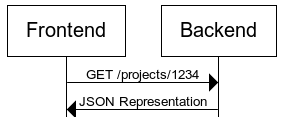
\includegraphics{figures/rest.png}
\caption{Petición de detalles sobre el proyecto con el identificador
``1234''. \label{figures:rest}}
\end{figure}

Por lo tanto, para estructurar la API que expondrá el backend, se
definieron 2 tipos de objetos:

\begin{itemize}
\item
  Proyectos: es casi la base de todo. Cada proyecto contendrá los
  diferentes archivos y carpetas.
\item
  Archivos: esto se refiere a archivos y carpetas. Por la forma en la
  que se manipulan los archivos en el servidor y en el cliente, es más
  conveniente manejarlos de (casi) la misma forma. Esto último se
  refiere a la forma en la que se obtienen los archivos en el servidor,
  y las acciones que se realizan en ellos. Ambos archivos y carpetas se
  crean y eliminan, como también se renombran. La única diferencia
  substancial es que las carpetas no tienen contenido y no se actualizan
  como el resto de los archivos.
\end{itemize}

De esta forma, el frontend podrá consultar sobre listas de proyectos,
detalles sobre cada proyecto (o cualquier método que se exponga, como
ensamblar el proyecto) y manipular archivos.

\subsection{Frontend}

Se comenzará por definir los diferentes objetos que existirán en el
frontend. Se definirán diferentes modelos, colecciones y vistas, por lo
que se recomienda revisar la Sección \ref{section:object-definition}
para sus significados.

\subsubsection{Definición de Objetos}

\paragraph{Modelos y Colecciones}

A continuación se explicará a grandes rasgos los modelos y colecciones
que existirán en el frontend. Se tendrán modelos para los proyectos y
los archivos. Cada uno se encargará de comunicarse con el backend para
obtener los datos que le sean necesarios o bien para guardar los
cambios.

\begin{description}
\item[El modelo de proyecto]
Guardará el nombre de éste y una referencia a una colección de los
archivos que se encuentren en la raíz de su carpeta. Tendrá como
responsabilidades crear archivos y carpetas, ensamblar el proyecto e
iniciar el servidor de pruebas. Estas acciones se complementan con
llamadas al backend que realizan las tareas mismas.
\item[El modelo de archivo]
Se encargará de guardar el nombre y el contenido (en caso de que
corresponda) del archivo o carpeta al que represente, además de guardar
una referencia al proyecto al que pertenece y a una colección de
archivos en caso de ser un directorio. Tendrá como responabilidades
pedir su contenido, actualizarlo, renombrar y eliminar el archivo del
sistema. Todas estas acciones se complementan además con llamadas al
backend.
\item[La colección de archivos]
Tendrá como responsabilidad ordenar las listas de archivos una vez que
la haya obtenido (además de guardar una referencia a cada modelo de
archivo que le corresponda). Ordenar las listas de archivos es
importante pues el backend arroja una lista de archivos ordenada
alfabéticamente, pero, dado que archivos y directorios son considerados
de la misma forma en el backend, es necesario ordenar la lista de manera
que los directorios queden arriba. Esto facilita encontrar archivos para
el usuario.
\end{description}

Como se ve en la Figura \ref{figures:frontend-models}, instancias de un
proyecto tendrán una colección de archivos base (representando el
directorio raíz), y estas colecciones contendrán instancias de archivos
(que pueden ser archivos o carpetas). En caso de ser un directorio,
guardaría una instancia a una colección de archivos.

\begin{figure}[htbp]
\centering
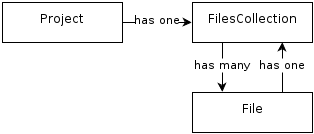
\includegraphics{figures/frontend-models.png}
\caption{Relaciones entre modelos y colecciones en el frontend.
\label{figures:frontend-models}}
\end{figure}

\paragraph{Vistas}

Cada una de las siguientes vistas considera un template asociado.

\begin{description}
\item[Explorador de Archivos]
Se colocará en la barra lateral izquierda, y tendrá dos listas de
archivos. Una lista de archivos actualmente abiertos y la lista de
archivos y directorios en el proyecto. Tendrá entre sus
responsabilidades mantener una lista de archivos que se encuentran
actualmente abiertos para que el usuario pueda navegar entre ellos.
\item[Archivo]
Esta vista representará a un archivo en la vista anterior (exporador de
archivos). Mostrará su nombre y un icono que represente si es un
directorio, un archivo o un template editable con el editor que se
construirá. Entre sus responsabilidades están abrir los archivos (o sea,
abrir el archivo en el editor de código o en el editor de vistas en caso
que corresponda), embeber listas de archivos en caso de que se clickee
un directorio y permitir al usuario renombrar archivos, mostrando un
menú contextual.
\item[Editor de Texto]
Esta vista contendrá el editor de archivos de texto (editor de código).
Sus responsabilidades serán mostrar un editor con resaltado de sintaxis
y modificar el modelo de archivo que corresponda para guardar cambios.
\item[Editor de Vistas]
Esta vista mostrará templates y, en una barra lateral derecha,
diferentes componentes para que el usuario los arrastre y agregue.
Contará además con un editor de código HTML, en caso de que el usuario
quiera editar la vista o realizar cambios que el editor no permita
directamente. Tiene las mismas responsabilidades que el editor de texto.
\end{description}

\subsubsection{Diseño del Editor de Templates}

El editor de interfaces se construirá de manera que el usuario pueda
arrastar componentes como botones o campos de texto directamente en una
vista previa del template que esté editando. El contenido de los
archivos de templates es simplemente HTML, por lo que es posible
presentarlos directamente en la aplicación. Este contenedor o vista
previa del template se le llamará ``canvas'' de ahora en adelante.

El objetivo es que el usuario arrastre elementos hacia el canvas de la
misma forma en la que se hace en Xcode o Visual Studio. El sistema debe
proveerle retroalimentación visual mostrando el objeto que está
arrastrando y además mostrar en qué lugar quedararía el elemento una vez
que el usuario lo suelte.

Para implementar este concepto de arrastrar y soltar, se utilizará
jQuery UI. esta librería provee, entre otras cosas, métodos para
habilitar el arrastrado de elementos en una página. El usuario
arrastrará un elemento, y, mediante las llamadas de jQuery, se colocará
el elemento en donde el usuario tenga su cursor en el momento, a manera
de proveer retroalimentación visual. En cuanto el usuario suelte el
elemento, se agregará su correspondiente fragmento de HTML en el
template, lo que se reflejará en el canvas en tiempo real.

\begin{figure}[htbp]
\centering
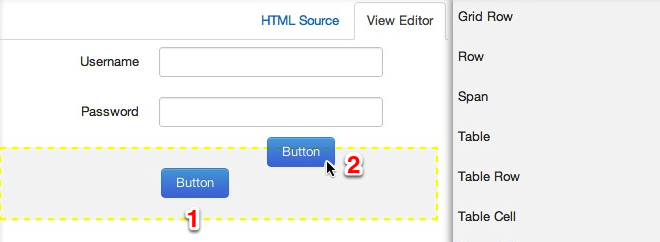
\includegraphics{figures/drag-editor.png}
\caption{Los diferentes elementos de retroalimentación visual que se
presentarían al arrastrar un componente. \label{figures:drag-editor}}
\end{figure}

En la Figura \ref{figures:drag-editor} se pueden apreciar los diferentes
elementos de retroalimentación al momento de arrastrar un elemento. En
el punto 1 se pueden ver, primero, un borde amarillo alrededor del
elemento en donde ``caería'' el componente. Además, en el mismo número,
puede visualizarse cómo se vería el componente (en este caso un botón)
una vez que el usuario lo deje ahí. En el número 2, puede verse el mismo
componente, que sigue al cursor mientras el usuario esté arrastrando.
Esto le muestra al usuario qué es lo que está arrastrando.

De esta forma, el desarrollador puede ver, por un lado, qué componente
estaría agregando al canvas y, por otro lado, cómo quedaría éste una vez
que lo agregue.

\section{Construcción de la Base}

\label{section:first-stage}

\subsection{Creación del Entorno de Trabajo}

En esta sección se detallarán cómo se crearon y estructuraron los dos
entornos de trabajo, tanto para el backend como para el frontend.

Ambos entornos de trabajo se crearon en carpetas independientes (dada su
naturaleza) y se inicializaron repositorios Git en cada una, a manera de
mantener un control de versiones en cada una.

\subsubsection{Entorno de Trabajo para el Backend}

El backend utilizará Ruby con Sinatra. Sinatra se diferencia de, por
ejemplo, Rails, en que es un framework mucho más simple. Por esto, es
que no posee utilidades para crear directorios de trabajo. La idea
detrás de Sinatra es crear todo en un sólo archivo. Si bien esto es
posible, e incluso aconsejable para algunas aplicaciones, no lo es para
ésta, en donde se tendrán diferentes modelos y controladores. Por lo
tanto se definió la siguiente estructura para el backend:

\begin{itemize}
\item
  \texttt{api}

  \begin{itemize}
  \item
    \texttt{v1}

    \begin{itemize}
    \item
      \texttt{config}: contiene diferentes archivos de configuración
    \item
      \texttt{controllers}: los diferentes controladores
    \item
      \texttt{models}: los modelos de usuario y proyecto
    \item
      \texttt{app.rb}: este archivo es la base de la aplicación Sinatra,
      pues nicializa ciertas configuraciones y contiene métodos
      compartidos por los controladores
    \item
      \texttt{boot.rb}: este archivo es cargado inicialmente y se
      encarga de incluir las diferentes librerías y archivos para
      incializar el servidor
    \end{itemize}
  \end{itemize}
\item
  \texttt{projects}: será el contenedor de los diferentes proyectos que
  crearán los usuarios
\item
  \texttt{public}: esta carpeta sirve archivos estáticos directamente,
  como imágenes
\item
  \texttt{Gemfile}: archivo utilizado por Bundler {[}41{]} para definir
  qué librerías y en qué versiones utilizará el backend
\item
  \texttt{config.ru}: archivo utilizado para levantar el servidor
\end{itemize}

Se decidió estructurar el backend en carpetas de versiones. La idea
detrás de esto es poder dividir cada versión de la API de manera de no
perder compatibilidad con posibles clientes que estén basados en una
versión de la API. Por ejemplo, de llegar a crearse un cliente para
tablets, cada cliente estaría atado a una versión específica. Si se
cambiara algún método (o se descontinuara), el cliente automáticamente
fallaría. En cambio, teniendo diferentes versiones, se puede mantener
esta compatibilidad.

Se creó además una carpeta llamada \texttt{projects}. Esta carpeta (que
no es accesible directamente), guarda cada uno de los proyectos de cada
usuario. Cada vez que se inicialice uno nuevo, se creará una subcarpeta
en este directorio con la estructura determinada.

El archivo \texttt{Gemfile} es un archivo que utiliza la librería
Bundler. Esta utilidad permite especificar librerías externas que se
quieren incluir en un proyecto (en este caso el backend) y especificar
sus versiones. Por ejemplo, un extracto de un archivo Gemfile podría
verse así:

\begin{Shaded}
\begin{Highlighting}[]
\NormalTok{gem }\StringTok{'sinatra'}\NormalTok{, }\StringTok{'1.3.3'} \CommentTok{# Especifica que se utilizará la versión 1.3.3}

\NormalTok{gem }\StringTok{'activerecord'}\NormalTok{, }\StringTok{'~> 3.2'} \CommentTok{# Especifica que se utilizarán }
                             \CommentTok{# versiones 3.2.X}

\NormalTok{gem }\StringTok{'haml'} \CommentTok{# Especifica que se utilizará la última versión}
\end{Highlighting}
\end{Shaded}

La gran utilidad de esta herramienta es que, al momento de ejecutar en
la consola \texttt{bundle install}, las versiones especificadas son
descargadas y se crea un archivo llamado \texttt{Gemfile.lock} que
guarda las versiones que están siendo utilizadas. De esta forma, cuando
otro desarrollador descargue el repositorio y ejecute nuevamente
\texttt{bundle install} para instalar las dependencias, se descargarán
exactamente esas versiones y ambos desarrolladores tendrán el mismo
entorno de desarrollo.

Finalmente, el archivo \texttt{config.ru} especifica cómo debe
levantarse el servidor. Este archivo detalla diferentes rutas que deben
ser ``montadas'' y a las cuales el servidor debe responder de diferentes
maneras. En este caso, se tendrán dos rutas (incialmente). Una, en la
que se montará el backend mismo, o sea, \texttt{/api/v1}, y la otra, en
la que se montará un servidor estático que sirva los archivos en la
carpeta \texttt{public}.

\subsubsection{Entorno de Trabajo para el Frontend}

De la misma forma en que Switch utilizará Brunch para crear y
administrar proyectos, se decidió utilizar la misma solución para
construir la IDE. Brunch utiliza un sistema de esqueletos
(``skeletons'', en inglés), los cuales utiliza para crear la estructura
de los proyectos. Existe una gran variedad, utilizando diferentes
lenguajes y frameworks. Se encontró uno que utiliza Backbone y
CoffeeScript y se utilizó para crear la estructura de archivos inicial.

De no existir esta estructura, habría que escribir todo dentro de un
sólo archivo, lo que para aplicaciones muy pequeñas puede ser práctico,
pero no lo es en este caso. La estructura consiste en la siguiente:

\begin{itemize}
\item
  \texttt{app}

  \begin{itemize}
  \item
    \texttt{assets}: imágenes y el archivo HTML principal de la
    aplicación
  \item
    \texttt{models}: los modelos y colecciones
  \item
    \texttt{routers}: definen los diferentes estados de la aplicación e
    inicializan lo necesario para funcionar en cada uno
  \item
    \texttt{styles}: archivos de estilo (CSS) modularizados para cada
    sección de la aplicación
  \item
    \texttt{views}: las vistas (o controladores)

    \begin{itemize}
    \item
      \texttt{templates}: los archivos con HTML de cada vista
    \end{itemize}
  \end{itemize}
\item
  \texttt{vendor}: librerías (Javascript o CSS) externas, como jQuery,
  Bootstrap, etc.
\end{itemize}

Existen otras carpetas que acá no se mencionan dado que no son
relevantes a la aplicación. La funcionalidad de cada uno de estos tipos
de archivos se explicaron en la Sección \ref{section:object-definition}.

Para crear el entorno de trabajo, simplemente se ejecuta el siguiente
comando:

\begin{verbatim}
brunch new -s git://github.com/meleyal/brunch-crumbs.git
\end{verbatim}

Este comando utiliza el esqueleto presente en
\href{https://github.com/meleyal/brunch-crumbs}{github.com/meleyal/brunch-crumbs}
para crear un directorio con la estructura ya mencionada.

\subsection{Prototipado de la Interfaz}

\label{section:prototyping}

Se comenzó por prototipar la interfaz principal. Como ya se ha dicho, se
utilizó Twitter Bootstrap, lo que permitió simplificar considerablemente
esta etapa. Para hacer el prototipado se requirió realizar un poco de
programación, pues hubo que crear vistas y rutas para ir testeando los
casos de uso definidos anteriormente. La programación fue mínima de
todas formas, enfocando esta etapa en prototipado y no en funcionalidad.

Se prototipó un menú superior con diferentes opciones de manera similar
a los menú que se ven en diferentes IDE y programas de escritorio. Se
incluyeron opciones como crear un nuevo proyecto, un nuevo archivo,
ensamblar y ejecutar el proyecto, etc.

Se agregó la barra lateral izquierda, en la que se muestra una lista de
los archivos abiertos y una lista de los archivos en el proyecto. Las
carpetas cuentan con un ícono que las muestra como tal, mientras que
archivos de templates tienen un ícono que los diferencia de las demás.
En la Figura \ref{figures:sidebar} pueden verse los diferentes íconos.

\begin{figure}[htbp]
\centering
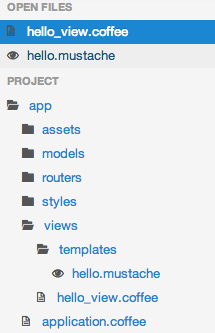
\includegraphics{figures/sidebar.png}
\caption{La barra lateral, en la que se pueden apreciar los íconos por
carpeta y archivo. \label{figures:sidebar}}
\end{figure}

Para el editor de código central se utilizó CodeMirror {[}42{]}.
CodeMirror es un widget que permite editar código en el navegador con
resaltado de sintaxis, líneas numeradas, entre otras características. El
editor de código se colocó en la parte central de la interfaz, como
puede verse en el recuadro rojo de la Figura \ref{figures:codemirror}.

\begin{figure}[htbp]
\centering
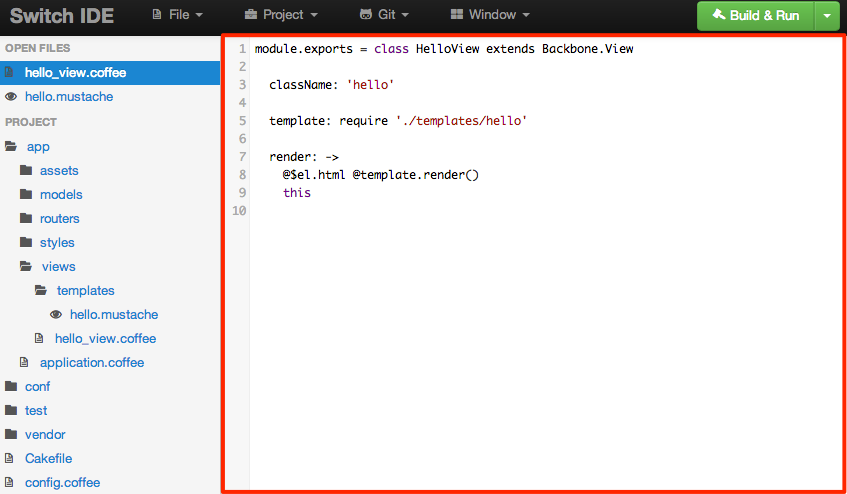
\includegraphics{figures/codemirror.png}
\caption{El recuadro rojo muestra cómo se ve CodeMirror al mostrar
código en CoffeeScript. Puede apreciarse el resaltado de sintaxis y las
líneas numeradas. \label{figures:codemirror}}
\end{figure}

En el caso del editor de vistas, se agregó un ``canvas'' (básicamente un
espacio en el cual arrastrar los componentes que se mencionarán más
adelante), y una barra lateral derecha, que sólo es visible al estar
editando un archivo que la requiera. Además del canvas, en la parte
superior se agregaron dos pestañas, que permitirán al usuario cambiar
entre el canvas y un editor de código para la vista. En la barra lateral
estarán los diferentes componentes en una lista que mostrará una pequeña
vista previa del componente y su nombre. En la Figura
\ref{figures:canvas} pueden apreciarse el canvas (número 1) y la barra
lateral con widgets (número 2).

\begin{figure}[htbp]
\centering
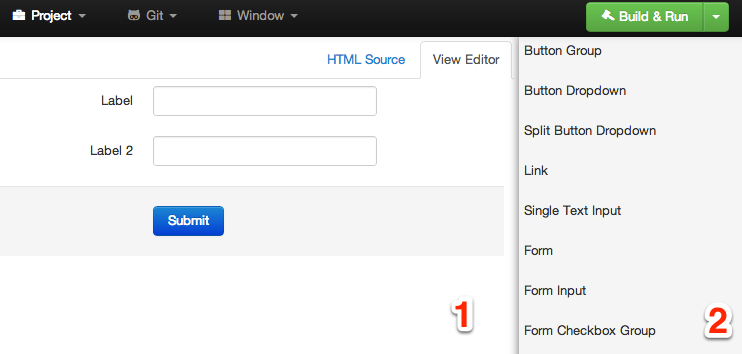
\includegraphics{figures/canvas.png}
\caption{El canvas a la izquierda (1), con los diferentes widgets
disponibles a la derecha (2). \label{figures:canvas}}
\end{figure}

La última vista corresponde al selector de proyectos (ver Figura
\ref{figures:projects-view}), que se creó usando una ventana modal (un
widget de Twitter Bootstrap). Ésta se mostraría en el momento que el
usuario ingrese al programa. Ahí, podrá elegir algún proyecto en el que
haya estado trabajando o crear uno nuevo directamente.

\begin{figure}[htbp]
\centering
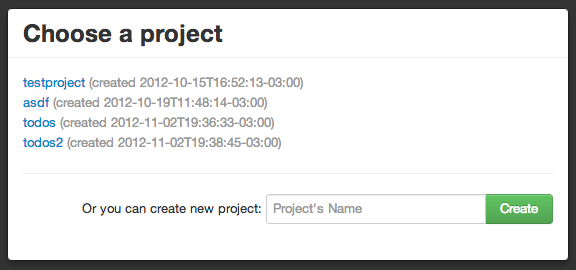
\includegraphics{figures/projects-view.png}
\caption{La ventana modal de selección de proyectos.
\label{figures:projects-view}}
\end{figure}

\subsection{Creación de Servicios en el Backend}

\label{section:create-services}

En las subsecciones siguientes se discutirán algunas de las
implementaciones de funcionalidades en el backend. Sin embargo no se
discutirán los métodos que se publican y son accesibles a través de la
API. Éstos últimos simplemente arrojan respuestas con objetos JSON como
el que sigue para comunicarse con el frontend, por lo que no se
considera necesario entrar en mucho detalle.

El siguiente es un fragmento de una respuesta del servidor al pedir los
archivos en el directorio raíz de un projecto.

\begin{Shaded}
\begin{Highlighting}[]
\NormalTok{[}
    \NormalTok{\{}
        \DataTypeTok{"name"}\NormalTok{: }\StringTok{"app"}\NormalTok{,}
        \DataTypeTok{"parent"}\NormalTok{: }\StringTok{""}\NormalTok{,}
        \DataTypeTok{"type"}\NormalTok{: }\StringTok{"directory"}
    \NormalTok{\},}
    \NormalTok{\{}
        \DataTypeTok{"name"}\NormalTok{: }\StringTok{"Cakefile"}\NormalTok{,}
        \DataTypeTok{"parent"}\NormalTok{: }\StringTok{""}\NormalTok{,}
        \DataTypeTok{"type"}\NormalTok{: }\StringTok{"file"}
    \NormalTok{\},}
    \NormalTok{\{}
        \DataTypeTok{"name"}\NormalTok{: }\StringTok{"conf"}\NormalTok{,}
        \DataTypeTok{"parent"}\NormalTok{: }\StringTok{""}\NormalTok{,}
        \DataTypeTok{"type"}\NormalTok{: }\StringTok{"directory"}
    \NormalTok{\},}
    \NormalTok{\{}
        \DataTypeTok{"name"}\NormalTok{: }\StringTok{"config.coffee"}\NormalTok{,}
        \DataTypeTok{"parent"}\NormalTok{: }\StringTok{""}\NormalTok{,}
        \DataTypeTok{"type"}\NormalTok{: }\StringTok{"file"}
    \NormalTok{\}}
    \ErrorTok{//} \ErrorTok{etc...}
\NormalTok{]}
\end{Highlighting}
\end{Shaded}

\subsubsection{Creación de Proyectos}

La creación de un proyecto nuevo es relativamente simple. Consiste en
crear un nuevo proyecto en la base de datos con el nombre que provee el
usuario, y luego crear el proyecto mismo utilizando Brunch.

Al crear un proyecto nuevo, el modelo guarda en la base de datos una
nueva entrada que está asociada al usuario que hace la llamada a la API.
Guarda un nombre para el proyecto, la ruta en la que fue guardado el
esqueleto y un puerto único. Antes de guardar la entrada en la base de
datos, un ``callback'' es gatillado en el mismo modelo (en Ruby) que
ejecuta el comando que crea la carpeta para el proyecto, como se detalla
a continuación:

\begin{Shaded}
\begin{Highlighting}[]
\KeywordTok{def} \NormalTok{create_project}
  \CommentTok{# Create a random path and the project}
  \DecValTok{self}\NormalTok{.path = }\StringTok{"}\OtherTok{#\{}\DecValTok{self}\NormalTok{.name}\OtherTok{\}}\StringTok{-}\OtherTok{#\{}\DataTypeTok{SecureRandom}\NormalTok{.hex(}\DecValTok{10}\NormalTok{)}\OtherTok{\}}\StringTok{"}
  \NormalTok{system }\StringTok{"brunch new }\OtherTok{#\{}\DecValTok{self}\NormalTok{.full_path}\OtherTok{\}}\StringTok{ \textbackslash{}}
\StringTok{          -s git://github.com/ianmurrays/brunch-crumbs.git"}
\KeywordTok{end}
\end{Highlighting}
\end{Shaded}

Se crea un sufijo aleatorio para evitar colisiones con proyectos que
tengan el mismo nombre, y se llama a un comando de sistema para crear el
esqueleto. Esta implementación no es perfecta, dado que podría darse el
caso de que \texttt{SecureRandom.hex(10)} arroje una cadena aleatoria
idéntica a alguna anterior. Para efectos del desarrollo del presente
trabajo, se decidió no darle demasiada importancia a este defecto, dado
que las probabilidades de que ello ocurra son demasiado bajas.

Después de que finalice este comando, se llama a un segundo ``callback''
que crea el número de puerto único para esta aplicación:

\begin{Shaded}
\begin{Highlighting}[]
\KeywordTok{def} \NormalTok{randomize_port}
  \KeywordTok{begin}
    \DecValTok{self}\NormalTok{.port = }\DecValTok{8000} \NormalTok{+ rand(}\DecValTok{2000}\NormalTok{)}
  \KeywordTok{end} \KeywordTok{until} \DataTypeTok{Project}\NormalTok{.where(port: }\DecValTok{self}\NormalTok{.port).count == }\DecValTok{0}
\KeywordTok{end}
\end{Highlighting}
\end{Shaded}

Básicamente asigna un puerto entre 8000 y 10000 aleatorio (y único) a
cada proyecto. De esta forma, si se están editando dos proyectos
simultáneamente, pueden levantarse dos instancias para hacer pruebas sin
colisionar. Esta implementación, si bien es suficiente para el
desarrollo de la herramienta y para este trabajo, no sería una
implementación ideal en producción, dado que alguno de esos puertos
podría estar siendo ocupado por algún servicio en el sistema. En una
futura implementación podría agregarse algún mecanismo que verifique la
disponibilidad del puerto al momento de asignarlo, o bien, verifique y
asigne puertos cada vez que se ensamble y corra el proyecto.

\subsubsection{Manipulación de Archivos}

La manipulación de archivos se hace directamente sobre ellos usando
librerías estándar de Ruby. Sólo se discutirán algunas de las
implementaciones presentes en el backend.

Para listar los archivos presentes en una determinada ruta, se utilizó
la siguiente implementación:

\begin{Shaded}
\begin{Highlighting}[]
\KeywordTok{def} \NormalTok{files_in(folder = }\StringTok{""}\NormalTok{)}
  \CommentTok{# Remove leading and trailing slashes}
  \NormalTok{folder.gsub! }\OtherTok{/^\textbackslash{}//}\NormalTok{, }\StringTok{""}
  \NormalTok{folder.gsub! }\OtherTok{/\textbackslash{}/$/}\NormalTok{, }\StringTok{""}

  \NormalTok{files = }\DataTypeTok{Dir}\NormalTok{[}\StringTok{"}\OtherTok{#\{}\DecValTok{self}\NormalTok{.full_path}\OtherTok{\}}\StringTok{/}\OtherTok{#\{}\NormalTok{folder}\OtherTok{\}}\StringTok{/*"}\NormalTok{].collect }\KeywordTok{do} \NormalTok{\textbar{}entry\textbar{}}
    \KeywordTok{next} \KeywordTok{if}\OtherTok{ %w\{}\StringTok{server.js node_modules}\OtherTok{\}}\NormalTok{.include? }\DataTypeTok{File}\NormalTok{.basename(entry)}
    \DecValTok{self}\NormalTok{.file_to_hash entry, folder}
  \KeywordTok{end}
\KeywordTok{end}
\end{Highlighting}
\end{Shaded}

El método lista todos los archivos presentes en la ruta especificada. De
no especificarse, lista los archivos en la raíz del proyecto. Primero se
eliminan las barras (\texttt{/}) al principio y final de la ruta que se
especifique, y luego se recorre el directorio usando la clase
Dir\footnote{Http://ruby-doc.org/core-1.9.3/Dir.html.}. La llamada a
\texttt{Dir{[}"/ruta/a/directorio"{]}} retorna un array que se recorre
utilizando \texttt{collect}. El método \texttt{collect} en los arreglos
genera un nuevo arreglo con los elementos que retorne el bloque que se
le pase. \texttt{collect} pasa cada elemento del arreglo original al
bloque como argumento para su manipulación. Por ejemplo, si el siguiente
fragmento de código retorna un nuevo arreglo con sus elementos elevados
al cuadrado:

\begin{Shaded}
\begin{Highlighting}[]
\NormalTok{[}\DecValTok{1}\NormalTok{,}\DecValTok{2}\NormalTok{,}\DecValTok{3}\NormalTok{,}\DecValTok{4}\NormalTok{,}\DecValTok{5}\NormalTok{].collect }\KeywordTok{do} \NormalTok{\textbar{}num\textbar{}}
  \NormalTok{num * num}
\KeywordTok{end}

\CommentTok{# => [1,4,9,16,25]}
\end{Highlighting}
\end{Shaded}

Por lo tanto, la variable \texttt{files} en la implementación de
\texttt{files\_in} contendrá la representación en un Hash\footnote{Http://www.ruby-doc.org/core-1.9.3/Hash.html.}
(básicamente un diccionario) de cada archivo (o directorio). Además, se
excluirán el directorio \texttt{node\_modules} y el archivo
\texttt{server.js} del listado, dado que son un directorio y un archivo
que no deben ser manipulados por el desarrollador.

La implementación del método \texttt{file\_to\_hash} es relativamente
simple, y genera un diccionario con el nombre, padre y tipo de archivo
para la ruta que se le pase como parámetro:

\begin{Shaded}
\begin{Highlighting}[]
\KeywordTok{def} \NormalTok{file_to_hash(file, folder)}
  \NormalTok{\{}
    \StringTok{:name} \NormalTok{=> }\DataTypeTok{File}\NormalTok{.basename(file),}
    \StringTok{:parent} \NormalTok{=> folder,}
    \StringTok{:type} \NormalTok{=> }\KeywordTok{if} \DataTypeTok{File}\NormalTok{.directory?(file)}
      \StringTok{:directory}
    \KeywordTok{else}
      \StringTok{:file}
    \KeywordTok{end}
  \NormalTok{\}}
\KeywordTok{end}
\end{Highlighting}
\end{Shaded}

Para obtener y actualizar el contenido de archivos se utilizó una
implementación relativamente simple:

\begin{Shaded}
\begin{Highlighting}[]
\KeywordTok{def} \NormalTok{file_content(path)}
  \KeywordTok{if} \DataTypeTok{FileTest}\NormalTok{.exists? }\DecValTok{self}\NormalTok{.full_path(path) \textbackslash{}}
     \KeywordTok{and}\NormalTok{ ! }\DataTypeTok{File}\NormalTok{.directory? }\DecValTok{self}\NormalTok{.full_path(path)}
    \NormalTok{\{}
      \StringTok{:content} \NormalTok{=> }\DataTypeTok{File}\NormalTok{.read(}\DecValTok{self}\NormalTok{.full_path(path))}
    \NormalTok{\}}
  \KeywordTok{end}
\KeywordTok{end}
\end{Highlighting}
\end{Shaded}

Básicamente, se verifica que el archivo indicado exista y que no sea un
directorio, y se retorna un Hash indicando el contenido del archivo. Se
decidió retornar un Hash pues facilita su lectura en el frontend,
retornando un objeto JSON en vez del contenido directamente.

Para la escritura de archivos se utilizó una implementación similar:

\begin{Shaded}
\begin{Highlighting}[]
\KeywordTok{def} \NormalTok{update_file(path, content)}
  \KeywordTok{if} \DataTypeTok{FileTest}\NormalTok{.exists? }\DecValTok{self}\NormalTok{.full_path(path) \textbackslash{}}
     \KeywordTok{and}\NormalTok{ ! }\DataTypeTok{File}\NormalTok{.directory? }\DecValTok{self}\NormalTok{.full_path(path)}
    \DataTypeTok{File}\NormalTok{.open(}\DecValTok{self}\NormalTok{.full_path(path), }\StringTok{'w'}\NormalTok{) }\KeywordTok{do} \NormalTok{\textbar{}file\textbar{}}
      \NormalTok{file.write content}
    \KeywordTok{end}
  \KeywordTok{end}
\KeywordTok{end}
\end{Highlighting}
\end{Shaded}

Se realiza la misma verificación que al momento de obtener el contenido.
Si el archivo existe y no es una carpeta, se reemplaza todo el contenido
directamente.

El renombrado de archivos y carpetas se realiza con el siguiente método:

\begin{Shaded}
\begin{Highlighting}[]
\KeywordTok{def} \NormalTok{rename_file(path, new_path)}
  \KeywordTok{if} \DataTypeTok{FileTest}\NormalTok{.exists? }\DecValTok{self}\NormalTok{.full_path(path)}
    \DataTypeTok{File}\NormalTok{.rename }\DecValTok{self}\NormalTok{.full_path(path), }\DecValTok{self}\NormalTok{.full_path(new_path)}
  \KeywordTok{end}

  \NormalTok{directory = }\DataTypeTok{File}\NormalTok{.split(new_path).first}

  \DecValTok{self}\NormalTok{.file_to_hash }\DecValTok{self}\NormalTok{.full_path(new_path), directory}
\KeywordTok{end}
\end{Highlighting}
\end{Shaded}

Se le pasan la ruta actual y la ruta nueva del archivo, y se devuelve la
nueva representación de éste para actualizar el modelo en el frontend.
La llamada a \texttt{File.rename} permite no sólo renombrar el archivo o
directorio, sino que además permite cambiar su ruta.

\subsubsection{Ensamblado y Servidor de Pruebas}

Para realizar el ensamblado se utiliza Brunch. De manera muy similar a
la creación de proyectos, es necesario ejecutar un comando de terminal
desde Ruby. La diferencia con la creación, es que acá se necesita leer
la salida del comando de manera de detectar si el ensamblado fue exitoso
o no. Para esto, se utiliza un comando distinto de \texttt{system} como
se vio antes.

\begin{Shaded}
\begin{Highlighting}[]
\KeywordTok{def} \NormalTok{build_project}
  \NormalTok{output, result = ::}\DataTypeTok{Open3}\NormalTok{.capture2e }\StringTok{"cd }\OtherTok{#\{}\DecValTok{self}\NormalTok{.full_path}\OtherTok{\}}\StringTok{ && brunch build"}

  \NormalTok{\{}
    \StringTok{:output} \NormalTok{=> output,}
    \StringTok{:result} \NormalTok{=> (output =~ }\OtherTok{/error/} \NormalTok{\textbar{}\textbar{} ! (output =~ }\OtherTok{/compiled/}\NormalTok{))}
  \NormalTok{\}}
\KeywordTok{end}
\end{Highlighting}
\end{Shaded}

La librería Open3\footnote{Http://www.ruby-doc.org/stdlib-1.9.3/libdoc/open3/rdoc/Open3.html.}
ejecutar comandos en el terminal con mayor flexibilidad. Dentro de los
comandos que provee está \texttt{capture2e}, que devuelve el output de
\texttt{stdout}y \texttt{stderr} combinados. Esto es útil en esta
situación dado que el ensamblado puede ser exitoso como no. De esta
forma, se ejecuta el comando \texttt{brunch build}, y se revisa su
output. Si éste contiene ``error'' o no contiene ``compiled'', significa
que ocurrió algún error, y el output se envía al frontend para que sea
mostrado.

Para ejecutar el servidor, se utiliza un acercamiento similar:

\begin{Shaded}
\begin{Highlighting}[]
\KeywordTok{def} \NormalTok{run_project}
  \NormalTok{output, result = ::}\DataTypeTok{Open3}\NormalTok{.capture2e }\StringTok{"cd }\OtherTok{#\{}\DecValTok{self}\NormalTok{.full_path}\OtherTok{\}}\StringTok{ \textbackslash{}}
\StringTok{                   && forever stop server.js }\OtherTok{#\{}\DecValTok{self}\NormalTok{.port}\OtherTok{\}}\StringTok{ \textbackslash{}}
\StringTok{                   && forever start server.js }\OtherTok{#\{}\DecValTok{self}\NormalTok{.port}\OtherTok{\}}\StringTok{"}

  \NormalTok{\{}
    \StringTok{:output} \NormalTok{=> output,}
    \StringTok{:url} \NormalTok{=> }\StringTok{"}\OtherTok{#\{}\DataTypeTok{Api}\NormalTok{::}\DataTypeTok{V1}\NormalTok{::}\DataTypeTok{App}\NormalTok{.settings.run_url}\OtherTok{\}}\StringTok{:}\OtherTok{#\{}\DecValTok{self}\NormalTok{.port}\OtherTok{\}}\StringTok{"}\NormalTok{,}
    \StringTok{:result} \NormalTok{=> !(output =~ }\OtherTok{/Forever processing file/}\NormalTok{)}
  \NormalTok{\}}
\KeywordTok{end}
\end{Highlighting}
\end{Shaded}

Utilizando un programa llamado Forever {[}43{]}, se ejecuta un script
que ya se mencionó anteriormente (que además viene con el esqueleto
utilizado por brunch al crear el proyecto). Este script levanta un
servidor estático en el puerto que se especifique, y si la ejecución fue
exitosa se retorna la información necesaria al frontend.

\subsection{Agregado de Funcionalidad al Prototipo del Frontend}

\subsubsection{Selector de Proyectos}

Se comenzó por implementar el selector de proyectos. Para esto fue
necesario implementar el modelo y colección de proyectos. En esta etapa
fueron implementados de la forma más simple posible. Básicamente, se
crearon como dos clases que extienden a \texttt{Backbone.Model} y
\texttt{Backbone.Collection} respectivamente. Dado que Backbone está
diseñado para interactuar con APIs REST, no fue necesario configurar más
que la URL del backend y especificar que la colección corresponde a una
colección de Proyectos.

Luego de configurar el modelo y la colección, se agregó una ruta al
enrutador de Backbone. El enrutador lee la URL del navegador e
interpreta qué método llamar del enrutador. La idea es que se
especifiquen las URL necesarias para la navegación de la aplicación. En
el caso de esta solución, sólo existirán dos rutas principalmente. La
primera será la ruta base, donde se cargará el selector de proyectos del
cual se habla, y la segunda será la que tendrá cada proyecto. Por lo
tanto, se configuró la URL base, y, en el método que es llamado, se
inicializa la colección de proyectos.

\begin{Shaded}
\begin{Highlighting}[]
\NormalTok{routes}\KeywordTok{:}
  \StringTok{''}\KeywordTok{:} \StringTok{'index'}

\NormalTok{index}\KeywordTok{:} \FunctionTok{->}
  \CommentTok{# We load projects and show them on a modal window}
  \NormalTok{projects }\KeywordTok{=} \KeywordTok{new} \DataTypeTok{Projects}\KeywordTok{()}
  
  \NormalTok{projectsView }\KeywordTok{=} \KeywordTok{new} \DataTypeTok{ProjectsView}\KeywordTok{(}\NormalTok{collection}\KeywordTok{:} \NormalTok{projects}\KeywordTok{)}
  \NormalTok{$}\KeywordTok{(}\StringTok{'body'}\KeywordTok{).}\NormalTok{append projectsView}\KeywordTok{.}\NormalTok{render}\KeywordTok{().}\NormalTok{el}
  \NormalTok{$}\KeywordTok{(}\StringTok{"#}\CharTok{#\{}\NormalTok{projectsView.id}\CharTok{\}}\StringTok{"}\KeywordTok{).}\NormalTok{modal}
    \NormalTok{backdrop}\KeywordTok{:} \StringTok{'static'}
    \NormalTok{keyboard}\KeywordTok{:} \OtherTok{false}

  \NormalTok{projects}\KeywordTok{.}\NormalTok{fetch}\KeywordTok{()}
\end{Highlighting}
\end{Shaded}

En el fragmento de código anterior puede verse el método \texttt{index}
que es llamado en este punto. Luego, la colección es pasada a una vista.
Las vistas, como se explicó antes, son las encargadas de presentar datos
al usuario (por medio de templates). Esta vista, básicamente, presenta
una lista de proyectos y un formulario para crear uno nuevo (esta última
funcionalidad se creará en la segunda etapa), como puede apreciarse en
la Figura \ref{figures:projects-view}.

Al usuario hacer click en un proyecto existente, se llama a la segunda
ruta en el enrutador. Esta ruta, toma el identificador de proyecto de la
url (que tienen un formato estilo \texttt{proyects/IDENTIFICADOR}) e
instancia un proyecto usando ese identificador. Una vez que se haya
obtenido toda su información desde el servidor, se le asigna el modelo a
la aplicación (de manera que su instancia quede compartida) y se
inicializa el visor de archivos (que es una vista) con éste. La ruta se
muestra en el fragmento de código siguiente:

\begin{Shaded}
\begin{Highlighting}[]
\NormalTok{routes}\KeywordTok{:}
  \StringTok{''}\KeywordTok{:} \StringTok{'index'}
  \StringTok{'projects/:id'}\KeywordTok{:} \StringTok{'project'}

\NormalTok{index}\KeywordTok{:} \FunctionTok{->}
  \CommentTok{# Omitido por brevedad.}

\NormalTok{project}\KeywordTok{:} \FunctionTok{(id) ->}
  \NormalTok{app}\KeywordTok{.}\NormalTok{project }\KeywordTok{=} \KeywordTok{new} \DataTypeTok{Project}\KeywordTok{(}\NormalTok{id}\KeywordTok{:} \NormalTok{id}\KeywordTok{)}
  \NormalTok{app}\KeywordTok{.}\NormalTok{project}\KeywordTok{.}\NormalTok{fetch}
    \NormalTok{success}\KeywordTok{:} \FunctionTok{=>}
      \NormalTok{app}\KeywordTok{.}\NormalTok{filebrowser}\KeywordTok{.}\NormalTok{setModel app}\KeywordTok{.}\NormalTok{project}
      \NormalTok{Backbone}\KeywordTok{.}\NormalTok{Mediator}\KeywordTok{.}\NormalTok{pub }\StringTok{'status:set'}\KeywordTok{,} \StringTok{"Project Loaded"}

  \NormalTok{Backbone}\KeywordTok{.}\NormalTok{Mediator}\KeywordTok{.}\NormalTok{pub }\StringTok{'modal:hide'}
\end{Highlighting}
\end{Shaded}

El visor de archivos toma el modelo de proyecto y ``pide'' su carpeta
raíz. El modelo hace una petición al backend, y éste contesta con una
representación de cada archivo (o carpeta) del directorio raíz. La
respuesta a esta llamada se presentó en la Sección
\ref{section:create-services}.

El visor de archivos, instancia una vista de archivo por cada uno de los
documentos que responde el backend. La vista de archivo se encarga de
mostrar el nombre y tipo de archivo, y permitir al usuario clickearlo
para abrirlo o ver su contenido. En caso de que el archivo se trate de
un directorio, la vista de archivo se encarga de mostrar sus contenidos.
Esta parte resultó ser un poco complicada de implementar, dado que lo
que se necesita es básicamente mostrar el mismo tipo de vista que la
raíz del proyecto pero para un subproyecto. Lo que se hizo en este caso
es lo siguiente: cuando el usuario hace click en un directorio, se
instancia una colección de archivos con la ruta a ese directorio. Se
hace una petición al servidor para que entregue la lista de archivos en
esa carpeta y se instancian vistas de archivo para cada uno,
embebiéndolas en la misma vista del directorio que se acaba de clickear.
En la Figura \ref{figure:file-browser} se puede apreciar el concepto. La
carpeta \texttt{app} es una vista de archivo, y contiene todos los
archivos y carpetas dentro de su recuadro. Lo mismo pasa con el
directorio \texttt{models}.

\begin{figure}[htbp]
\centering
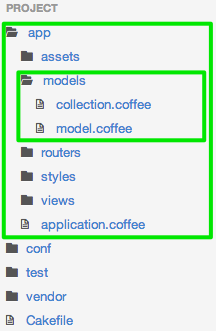
\includegraphics{figures/file-browser.png}
\caption{El visor de archivos: cada vista de directorio contiene más
vistas de archivos de ser necesarias. \label{figure:file-browser}}
\end{figure}

En caso de que el usuario haga click en un archivo, se le pasa la
instancia del modelo al editor de código, el cual indica al modelo que
debe pedir el contenido del archivo al servidor para mostrarlo. El
editor de código utiliza CodeMirror (ver Sección
\ref{section:prototyping}) y básicamente muestra el contenido del
archivo en el editor, que se encarga de formatearlo y resaltar sintaxis,
entre otras responsabilidades. El editor se encarga además de actualizar
el contenido del archivo al momento de guardar.

Para esta etapa de la construcción, se incluyó además la posibilidad de
ensamblar y ejecutar el proyecto. Para esto, se agregaron métodos en el
modelo de proyectos que hace llamadas al backend para ensamblar y
ejectuar el servidor de pruebas. El evento es manejado por la barra de
navegación, que incluye varios elementos de menú que por esta etapa se
mantuvieron inactivos. A la derecha de la barra de navegación se
encuentra un botón que permite ensamblar y ejecutar el proyecto con un
sólo click, y otros dos que permiten ejecutarlo y ensamblarlo por
separado.

En esta etapa se agregaron además atajos de teclado. Para esto se
utilizó una librería Javascript llamada Mousetrap {[}44{]}. Esta
librería permite configurar muy fácilmente atajos de teclado con una
gran flexibilidad en términos de combinaciones de teclas. Por ejemplo,
si se quisiera agregar un atajo de teclado para guardar el archivo
actual, se puede hacer lo siguiente:

\begin{Shaded}
\begin{Highlighting}[]
\NormalTok{Mousetrap}\KeywordTok{.}\NormalTok{bind }\KeywordTok{[}\StringTok{"ctrl+s"}\KeywordTok{,} \StringTok{"command+s"}\KeywordTok{],} \FunctionTok{->}
  \CommentTok{# Guardar el archivo}
\end{Highlighting}
\end{Shaded}

Esto permite que el usuario use la combinación ``CTRL+S'' o bien, en
computadores Mac, ``COMMAND+S''. Es posible agregar atajos de teclado
más complejos, como ``CTRL+ALT+S'' o ``CTRL+SHITF+S'', etc. Incluso, es
posible saber si el usuario está manteniendo presionada alguna tecla.
Por ejemplo, si se quiere saber si el usuario está manteniendo
presionada la tecla ``SHIFT'', se puede hacer de la siguiente forma:

\begin{Shaded}
\begin{Highlighting}[]
\NormalTok{Mousetrap}\KeywordTok{.}\NormalTok{bind }\KeywordTok{[}\StringTok{'shift'}\KeywordTok{],} \FunctionTok{(e) =>}
      \CommentTok{# El usuario está manteniendo presionada la tecla SHIFT}
    \KeywordTok{,} \StringTok{'keydown'}
\end{Highlighting}
\end{Shaded}

Utilizando esta librería, se agregaron varios atajos de teclado en esta
etapa. Entre ellos:

\begin{itemize}
\item
  Guardar archivo actual: \texttt{CTRL+S}
\item
  Cerrar el archivo actual: \texttt{CTRL+W}
\item
  Ejecutar el proyecto: \texttt{CTRL+R}
\item
  Cambiar entre archivos abiertos: \texttt{CTRL+NUMERO}
\end{itemize}

Este último atajo mencionado permite al usuario cambiar entre los
archivos que están abiertos en la lista de la derecha. La mayoría de los
editores de código permiten cambiar rápidamente entre los archivos
abiertos de esta manera.

Casi todos los atajos de teclado son interpretados por el navegador. Por
ejemplo, el atajo para guardar, para cambiar entre archivos abiertos,
todos ellos son atajos que el navegador utiliza internamente. Para
evitar que el navegador los intercepte, se utilizó la siguiente técnica:

\begin{Shaded}
\begin{Highlighting}[]
\NormalTok{Moustrap}\KeywordTok{.}\NormalTok{bind }\KeywordTok{[}\StringTok{"ctrl+s"}\KeywordTok{],} \FunctionTok{(event) ->}
  \NormalTok{event}\KeywordTok{.}\NormalTok{prevendDefault}\KeywordTok{()}
  
  \CommentTok{# Guardar el archivo}
\end{Highlighting}
\end{Shaded}

Cada ``evento'' que es generado en Javascript, normalmente es pasado a
los callbacks. En este caso, es posible llamar al método
\texttt{preventDefault()} del evento, lo que indica al navegador que no
realice la acción por defecto que debería. Si no se llamara a este
método, el archivo de todas formas se guardaría, pues el evento se está
llamando, pero el navegador también mostraría la ventana de ``Guardar
Página'' que por defecto aparecería en otro caso, y eso no es lo que se
quiere en una aplicación web de este estilo.

\section{Construcción del Editor de Interfaces}

\label{section:interface-editor}

El editor se diseñó de manera que en el centro se tuviera una vista en
vivo de lo que se estaba construyendo, mientras que a la derecha se
listaran todos los componentes disponibles para agregar al template.
Dado que los templates son básicamente HTML, es el navegador el que se
encarga de mostrar cómo se vería finalmente. Por esto, lo que se hizo
fue agregar elementos a la lista de componentes de manera que al
arrastrarlos hacia el centro (el editor), simplemente se agregue su
representación en HTML y el navegador se encargaría de mostrar su
``vista previa''.

Entonces, en la lista de componentes se decidió agregar botones, tablas,
formularios, campos de texto, entre otros, y dentro de ellos (en código,
no visible para el usuario) agregar un fragmento de HTML que se
agregaría al template. Luego, utilizando jQuery UI {[}45{]}, cada
componente se convierte en un elemento arrastrable. Con jQuery UI, se
necesita convertir elementos en ``arrastrables'' y además, crear
elementos en donde ``soltar'' lo que el usuario está arrastrando. En
este sentido, y, en un primer intento, se convierten todos los elementos
en la vista previa en ``soltables''.

\begin{Shaded}
\begin{Highlighting}[]
\CommentTok{# Con la siguiente llamada, se convierte cada elemento en el editor}
\CommentTok{# de vistas en "soltable".}
\NormalTok{@$}\KeywordTok{(}\StringTok{"*"}\KeywordTok{).}\NormalTok{droppable}\KeywordTok{()}
\end{Highlighting}
\end{Shaded}

Con este primer acercamiento, ya se podía arrastrar y soltar
componentes. El problema es que se podían arrastar componentes como
botones y otras cosas dentro de elementos HTML que no correspondía, como
imágenes, menús, etc. Para esto, se incluyeron ciertas excepciones a la
llamada anterior, como sigue:

\begin{Shaded}
\begin{Highlighting}[]
\CommentTok{# Seleccionar todos los elementos, excepto los que están en la}
\CommentTok{# llamada .not()}
\NormalTok{@$}\KeywordTok{(}\StringTok{"*"}\KeywordTok{).not(}\StringTok{'img, button, input, select, option, optgroup'}\KeywordTok{).}\NormalTok{droppable}\KeywordTok{()}
\end{Highlighting}
\end{Shaded}

Con esto, se simplificó un tanto el arrastrado de componentes, evitando
que algunos quedaran dentro de elementos que no correspondía. Ahora, se
notó que era difícil saber dónde realmente se estaba dejando el
componente que el usuario estaba arrastrando, por lo que se incluyó
retroalimentación visual al momento de arrastar, es decir, cuando el
usuario esté arrastrando el elemento, el elemento en donde ``caería'' el
componente se rodea con un borde amarillo, como muestra la Figura
\ref{figures:drag-editor}. Esto se logra usando propiedades de jQuery
UI:

\begin{Shaded}
\begin{Highlighting}[]
\NormalTok{exceptions }\KeywordTok{=} \StringTok{'img, button, input, select, option, optgroup'}
\NormalTok{@$}\KeywordTok{(}\StringTok{"*"}\KeywordTok{).not(}\NormalTok{exceptions}\KeywordTok{).}\NormalTok{droppable}
  \NormalTok{hoverClass}\KeywordTok{:} \StringTok{"hovering"} \CommentTok{# Esto agrega una clase CSS con un borde.}
\end{Highlighting}
\end{Shaded}

La propiedad \texttt{hoverClass} agrega una clase CSS al elemento donde
se estaría arrastrando el componente y la remueve al salir. Con esto se
agrega un borde que facilite al usuario saber dónde caerá el componente.

Se decidió además agregar componentes que sólo sirven si se arrastran
dentro de un formulario. En este punto, el usuario puede arrastrar estos
componentes a cualquier parte, lo que hace de su uso algo complicado.
Para solucionar esto, se implementó un sistema en el cual cada
componente tiene especificado dónde puede ser arrastrado. Por ejemplo,
los botones pueden ser arrastrados a cualquier parte:

\begin{Shaded}
\begin{Highlighting}[]
\KeywordTok{<div}\OtherTok{ class=}\StringTok{"switch-component"}\OtherTok{ data-component-type=}\StringTok{"button"}\KeywordTok{>}
  \KeywordTok{<div}\OtherTok{ class=}\StringTok{"payload"}\KeywordTok{>}
    \KeywordTok{<button}\OtherTok{ type=}\StringTok{"button"}\OtherTok{ class=}\StringTok{"btn btn-primary"}\KeywordTok{>}\NormalTok{Button}\KeywordTok{</button>}
  \KeywordTok{</div>}

  \KeywordTok{<span}\OtherTok{ class=}\StringTok{"name"}\KeywordTok{>}\NormalTok{Button}\KeywordTok{</span>}
\KeywordTok{</div>}
\end{Highlighting}
\end{Shaded}

En cambio, los elementos de un formulario sólo pueden arrastrarse a un
formulario previamente colocado. En el siguiente fragmento se puede
notar la propiedad \texttt{data-component-drop-only} que contiene una
cadena de texto con selectores CSS en dónde puede ser agregado.

\begin{Shaded}
\begin{Highlighting}[]
\KeywordTok{<div}\OtherTok{ class=}\StringTok{"switch-component"}\OtherTok{ data-component-type=}\StringTok{"label-button"} 
\OtherTok{     data-component-drop-only=}\StringTok{"form"}\KeywordTok{>}
  \KeywordTok{<div}\OtherTok{ class=}\StringTok{"payload"}\KeywordTok{>}
    \KeywordTok{<div}\OtherTok{ class=}\StringTok{"control-group"}\KeywordTok{>}
      \KeywordTok{<div}\OtherTok{ class=}\StringTok{"control-label"}\KeywordTok{><label}\OtherTok{ for=}\StringTok{"new_input"}\KeywordTok{>}\NormalTok{Label}\KeywordTok{</label></div>}
      \KeywordTok{<div}\OtherTok{ class=}\StringTok{"controls"}\KeywordTok{>}
        \KeywordTok{<input}\OtherTok{ type=}\StringTok{"text"}\OtherTok{ name=}\StringTok{"new_input"}\OtherTok{ id=}\StringTok{"new_input"}\KeywordTok{>}
      \KeywordTok{</div>}
    \KeywordTok{</div>}
  \KeywordTok{</div>}

  \KeywordTok{<span}\OtherTok{ class=}\StringTok{"name"}\KeywordTok{>}\NormalTok{Form Input}\KeywordTok{</span>}
\KeywordTok{</div>}
\end{Highlighting}
\end{Shaded}

Lo anterior, junto con el siguiente Coffeescript, permite que los
componentes puedan ser arrastrados sólo a ciertos elementos, si es que
lo especifican:

\begin{Shaded}
\begin{Highlighting}[]
\NormalTok{makeDroppable}\KeywordTok{:} \FunctionTok{(only) ->}
  \CommentTok{# Si se especificó only, entonces usarlo, de lo contrario}
  \CommentTok{# permitir cualquier elemento.}
  \KeywordTok{if} \NormalTok{only}
    \NormalTok{only }\KeywordTok{=} \StringTok{"#view_container }\CharTok{#\{}\NormalTok{only}\CharTok{\}}\StringTok{"}
  \KeywordTok{else}
    \NormalTok{only }\KeywordTok{=} \StringTok{"#view_container, #view_container *"}

  \NormalTok{@$}\KeywordTok{(}\NormalTok{only}\KeywordTok{).not(}\NormalTok{exceptions}\KeywordTok{).}\NormalTok{droppable}
    \NormalTok{hoverClass}\KeywordTok{:} \StringTok{"hovering"}
\end{Highlighting}
\end{Shaded}

Hasta ahora, el editor de templates agrega los componentes anexándolos
al final de la posición en la que el usuario las deja. Esto lo
imposibilita de agregar componentes al principio de una lista por
ejemplo. Por lo tanto, se agregoó la posibilidad de cambiar ese
comportamiento. Al momento de arrastrar un componente, el usuario puede
presionar (y mantener presionada) la tecla \texttt{SHIFT}, de manera que
al dejar un componente, éste se anexe al principio en vez de al final,
permitiendo al usuario agregar cosas al principio de listas o
formularios, por ejemplo.

Por último, para facilitar aún más el arrastrado de componentes, se
agregó una vista previa de cómo quedaría el componente que se está
arrastrando una vez que se suelte. La idea es que al estar arrastrando
un elemento, éste aparece en el editor con una ligera opacidad. Esto se
logró usando algunas llamadas de jQuery UI. Con estas llamadas, al
momento de que el usuario esté sobre un elemento (``over''),
literalmente se agrega el componente al editor, para luego eliminarlo en
caso de salirse (``out''), o bien dejarlo definitivamente al soltarlo
(``drop''). En la Figura \ref{figures:drag-editor} puede verse un
ejemplo de este comportamiento, y el fragmento de código asociado puede
verse a continuación:

\begin{Shaded}
\begin{Highlighting}[]
\CommentTok{# ...}
\NormalTok{@$}\KeywordTok{(}\NormalTok{only}\KeywordTok{).not(}\NormalTok{exceptions}\KeywordTok{).}\NormalTok{droppable}
  \NormalTok{hoverClass}\KeywordTok{:} \StringTok{"hovering"}
  \NormalTok{greedy}\KeywordTok{:} \OtherTok{yes}
  \NormalTok{drop}\KeywordTok{:} \FunctionTok{(e, u) ->} 
    \NormalTok{self}\KeywordTok{.}\NormalTok{putComponent}\KeywordTok{(}\NormalTok{self}\KeywordTok{,} \NormalTok{$}\KeywordTok{(}\DataTypeTok{this}\KeywordTok{),} \NormalTok{u}\KeywordTok{,} \OtherTok{no}\KeywordTok{)}
  \NormalTok{over}\KeywordTok{:} \FunctionTok{(e, u) ->}
    \NormalTok{self}\KeywordTok{.}\NormalTok{putComponent}\KeywordTok{(}\NormalTok{self}\KeywordTok{,} \NormalTok{$}\KeywordTok{(}\DataTypeTok{this}\KeywordTok{),} \NormalTok{u}\KeywordTok{,} \OtherTok{yes}\KeywordTok{)}
  \NormalTok{out}\KeywordTok{:} \FunctionTok{(e, u) ->} 
    \NormalTok{self}\KeywordTok{.}\NormalTok{removeComponent}\KeywordTok{()}
\end{Highlighting}
\end{Shaded}

Por último, el editor de templates también debería permitir al usuario
editar el código directamente, en caso de que no exista algún componente
o bien se necesite agregar cierta lógica más allá de HTML. Para esto, se
utilizó el mismo editor de código que para los archivos normales. Se
agregaron dos pestañas en la parte superior del editor de templates que
permiten cambiar entre el editor visual y el código fuente (ver Figura
\ref{figure:html-editor}).

\begin{figure}[htbp]
\centering
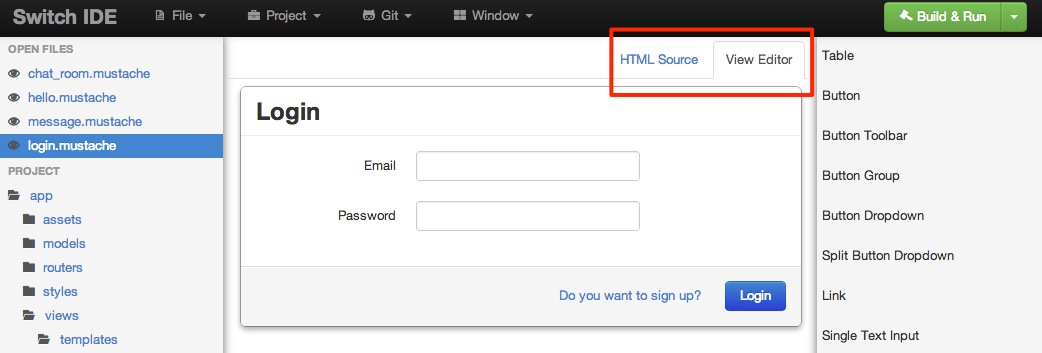
\includegraphics{figures/html-editor.png}
\caption{Las pestañas señaladas permiten al usuario cambiar entre el
modo visual y el editor HTML \label{figure:html-editor}}
\end{figure}

Por último, existe una propiedad en HTML5 que permite al usuario editar
cualquier parte de un sitio directo desde el navegador. Al habilitar
esta propiedad en el canvas, el usuario puede cambiar etiquetas de
formulario, o escribir directamente en el canvas sin tener que cambiar
al editor de HTML para agregar texto. Para habilitar esta propiedad,
basta con agregar el atributo \texttt{contenteditable} a la etiqueta del
canvas:

\begin{Shaded}
\begin{Highlighting}[]
\KeywordTok{<div}\OtherTok{ id=}\StringTok{"view_container"}\OtherTok{ contenteditable}\KeywordTok{>}
  \CommentTok{<!-- El canvas -->}
\KeywordTok{</div>}
\end{Highlighting}
\end{Shaded}

\clearpage
\newpage

\chapter{Resultados}

\label{sections:results}

\section{Producto Final}

La herramienta que se logró en este trabajo permite desarrollar
aplicaciones web completas en un navegador. Desde la creación del
proyecto hasta la edición y ejecución de la aplicación, la solución es
una IDE completa. Se logró incluir suficiente funcionalidad como para
considerarse la solución buscada.

El componente más importante de Switch, el editor de interfaces, logra
asemejarse bastante a lo que se puede encontrar en herramientas
similares, como Xcode u otras de las mencionadas en la Sección
\ref{section:state-of-the-art}. Es un editor de uso intuitivo y con una
gran cantidad de componentes presentes en Twitter Bootstrap, lo que
permite prototipar interfaces rápida y fácilmente.

Aun cuando el editor es de fácil uso, sigue estando apuntado a usuarios
expertos (desarrolladores específicamente), y no a diseñadores u otras
personas que deseen prototipar interfaces solamente. Por esto mismo es
que el editor provee un modo de edición de HTML, para que el
desarrollador pueda realizar cambios más ``finos'' en los templates que
edite, además de tener la posibilidad de agregar más componentes que no
estarían presentes en el listado.

Además, está la posibilidad de ensamblar y probar el proyecto desde la
misma IDE. El desarrollador puede simplemente presionar ``Build \& Run''
o usar el atajo de teclado \texttt{CMD+R} (\texttt{CTRL+R} en Windows y
Linux) para que el programa ensamble y levante el servidor con el
proyecto.

\section{Modo de Uso de la Herramienta}

En esta sección se describirá cómo utilizar la herramienta. Es
importante mencionar que la solución propuesta está pensada para
usuarios que ya tengan conocimientos para programar en Backbone, por lo
que no se explicará cómo desarrollar con este framework.

\subsection{Creación y Selección de Proyectos}

Al ingresar por primera vez, al desarrollador se le presenta la ventana
de selección de proyectos. En ella, se mostrarán los proyectos
existentes y un pequeño formulario que le permitirá crear un proyecto
nuevo.

Para abrir un proyecto existente, basta con clickear en uno de ellos
(número 1 de la Figura \ref{figures:tutorial-projects}). Si el usuario
deseara crear un proyecto nuevo, puede escribir el nombre de éste en el
formulario de abajo y presionar ``Create'' (número 2 de la Figura
\ref{figures:tutorial-projects}).

\begin{figure}[htbp]
\centering
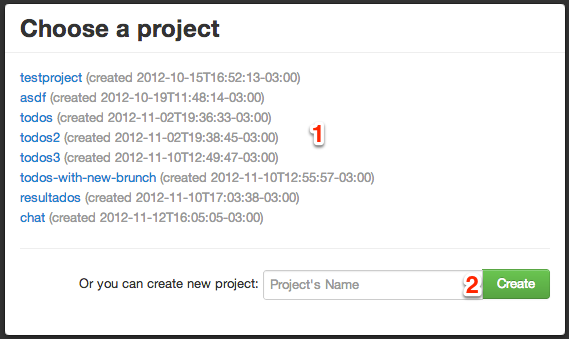
\includegraphics{figures/tutorial-projects.png}
\caption{El selector de proyectos. El usuario puede abrir un proyecto
existente (1) o crear uno nuevo (2). \label{figures:tutorial-projects}}
\end{figure}

En ambos casos, se abrirá el proyecto y el usuario será presentado con
la vista principal de la aplicación.

\subsection{Manejo de Archivos y Carpetas}

El usuario puede realizar acciones básicas sobre los archivos. Para
crear un archivo nuevo, basta con hacer click secundario sobre el
directorio donde se desee crear uno y seleccionar ``New File'' (ver
Figura \ref{figures:tutorial-new-file}). Se mostrará una ventana modal
en donde el usuario podrá escribir el nombre del archivo nuevo, como se
puede ver en la Figura \ref{figures:tutorial-new-file-prompt}. En caso
de que el usuario escoja un nombre que se encuentre en uso, el sistema
le alertará correspondientemente.

\begin{figure}[htbp]
\centering
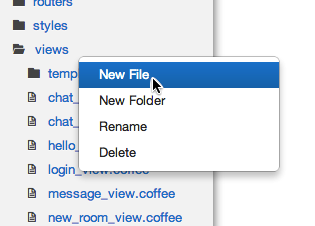
\includegraphics{figures/tutorial-new-file.png}
\caption{El menú contextual que aparece al hacer click derecho sobre un
archivo o directorio.\label{figures:tutorial-new-file}}
\end{figure}

\begin{figure}[htbp]
\centering
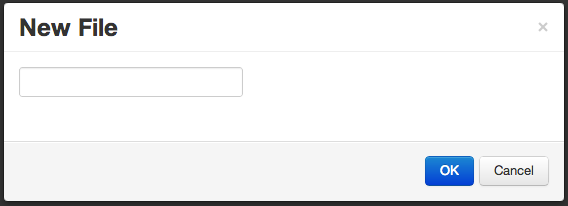
\includegraphics{figures/tutorial-new-file-prompt.png}
\caption{La ventana modal que permite al usuario escribir el nombre de
un archivo (o directorio)
nuevo.\label{figures:tutorial-new-file-prompt}}
\end{figure}

El procedimiento es casi idéntico para la creación de directorios, con
la única diferencia de que el usuario deberá escoger ``New Folder''
desde el menú contextual que se muestra en la Figura
\ref{figures:tutorial-new-file}.

Para renombrar archivos y directorios, se debe hacer click derecho sobre
éste y presionar ``Rename''. El nombre del archivo se convertirá en un
campo de texto donde el usuario podrá escribir el nombre nuevo. Para
finalizar el renombrado bastará con presionar la tecla ENTER. En la
Figura \ref{figures:tutorial-rename} puede verse el campo de texto que
aparece al renombrar un directorio.

\begin{figure}[htbp]
\centering
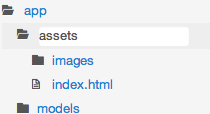
\includegraphics{figures/tutorial-rename.png}
\caption{Al renombrar un directorio o archivo aparece un campo de texto
para cambiar el nombre. \label{figures:tutorial-rename}}
\end{figure}

Para eliminar archivos y directorios, debe seleccionarse la opción
``Delete'' del menú contextual. Se presenta una confirmación,
especificando qué archivo o carpeta se eliminará, como se ve en la
Figura \ref{figures:tutorial-confirm}.

\begin{figure}[htbp]
\centering
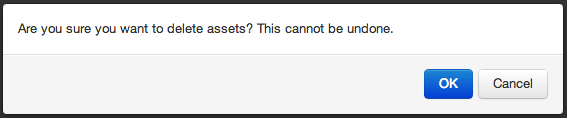
\includegraphics{figures/tutorial-confirm.png}
\caption{Se le pide confirmación al usuario antes de eliminar algún
archivo o carpeta. \label{figures:tutorial-confirm}}
\end{figure}

\subsection{Edición de Archivos}

Para abrir un archivo, se debe hacer click en él. Se cargará el editor
de código a la derecha, mostrando los contenidos de éste. Ahí, el
usuario puede hacer los cambios que sean necesarios. En la Figura
\ref{figures:tutorial-code} puede verse el editor de código al abrir un
archivo.

\begin{figure}[htbp]
\centering
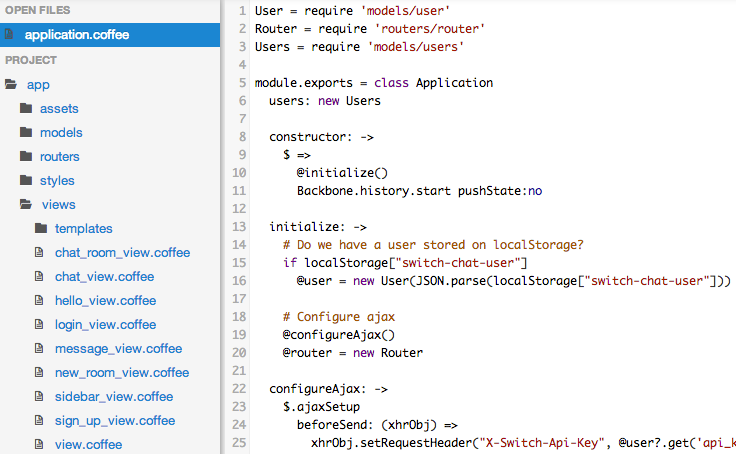
\includegraphics{figures/tutorial-code.png}
\caption{El editor de código al abrir el archivo
\texttt{application.coffee} de un proyecto.
\label{figures:tutorial-code}}
\end{figure}

Para guardar los cambios, el usuario puede presionar \texttt{CTRL+S} en
el teclado. Una vez que el archivo se haya guardado correctamente, se
verá un mensaje arriba a la derecha, en la barra de navegación (ver
Figura \ref{figures:tutorial-message}).

\begin{figure}[htbp]
\centering

\includegraphics{figures/tutorial-message.png}
\caption{Mensaje que aparece en la esquina superior derecha al guardarse
exitosamente un archivo. \label{figures:tutorial-message}}
\end{figure}

En caso de que el usuario abriera otro archivo sin antes haber guardado
los cambios, el sistema automáticamente guardará los cambios por él
antes de cambiar al siguiente archivo.

\subsection{Edición de Templates}

Cuando el usuario hace click en un template (archivos denotados con un
ícono específico en el explorador de archivos, ver Figura
\ref{figures:tutorial-template-icon}), se carga el editor de interfaces
en vez del editor de código simple.

\begin{figure}[htbp]
\centering
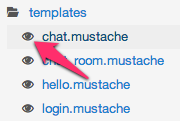
\includegraphics{figures/tutorial-template-icon.png}
\caption{El ícono que diferencia los archivos de código de los
templates. \label{figures:tutorial-template-icon}}
\end{figure}

El editor de interfaces muestra el contenido del template en vivo, y
permite al usuario arrastrar widgets de la barra lateral derecha hacia
el canvas. Por ejemplo, en la Figura \ref{figures:tutorial-drag}, puede
verse cómo se arrastra un componente llamado ``Prepended Input'' a un
formulario de registro en el canvas.

\begin{figure}[htbp]
\centering
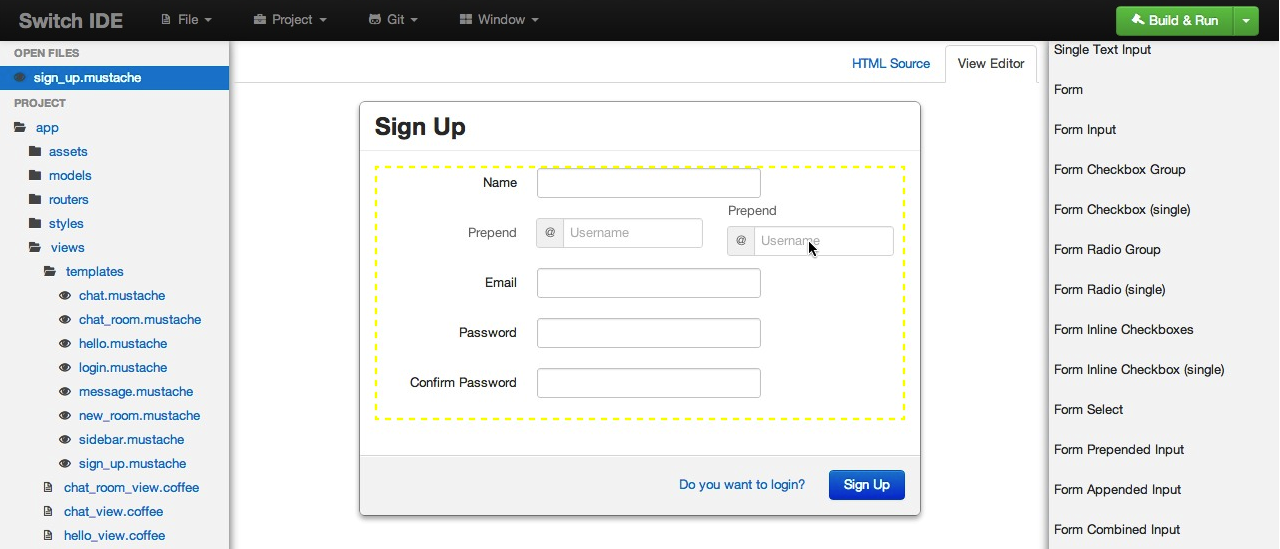
\includegraphics{figures/tutorial-drag.png}
\caption{Arrastrando un componente hacia un formulario de registro en el
editor de templates. \label{figures:tutorial-drag}}
\end{figure}

También es posible editar el HTML que se va generando con el editor. Por
ejemplo, en caso de que el desarrollador desee agregar un atributo de
clase o un identificador, puede hacerlo usando el editor de HTML. Para
acceder a él, es posible presionar las teclas
\texttt{CTRL+ALT+FLECHA ARRIBA} o bien utilizar las pestañas presentes
arriba del canvas (ver Figura \ref{figures:tutorial-html}).

\begin{figure}[htbp]
\centering
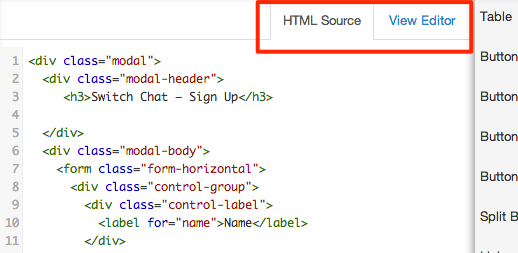
\includegraphics{figures/tutorial-html.png}
\caption{En el recuadro pueden verse las pestañas que permiten cambiar
entre el modo de edición de HTML y el editor visual.
\label{figures:tutorial-html}}
\end{figure}

\subsection{Ejecutar el Proyecto}

La ejecución del proyecto consiste en ensamblarlo y ejecutarlo. Existen
varias formas de hacer esto. Si se desea ensamblar y ejecutar el
proyecto de una vez, puede presionarse \texttt{CTRL+R} en el teclado o
bien presionar el botón ``Build \& Run'' en la esquina superior derecha.
En ambos casos, se mostrará el progreso en la misma esquina, como puede
verse en la Figura \ref{figures:tutorial-build}.

\begin{figure}[htbp]
\centering

\includegraphics{figures/tutorial-build.png}
\caption{El botón para ensamblar y ejecutar, junto con la barra de
progreso. \label{figures:tutorial-build}}
\end{figure}

En caso de necesitar sólamente ensamblar o ejecutar (de forma
independiente), es posible, clickeando la flecha al costado del botón
``Build \& Run''. Esto mostrará un menú contextual con ambas opciones,
como se ve en la Figura \ref{figures:tutorial-contextual}.

\begin{figure}[htbp]
\centering
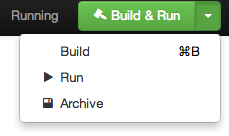
\includegraphics{figures/tutorial-contextual.png}
\caption{El menú contextual con las opciones para ensamblar, ejecutar y
archivar el proyecto. \label{figures:tutorial-contextual}}
\end{figure}

En caso de que el ensamblado falle, se mostrará una ventana con el
detalle del error, como se puede ver en la Figura
\ref{figures:tutorial-error}.

\begin{figure}[htbp]
\centering
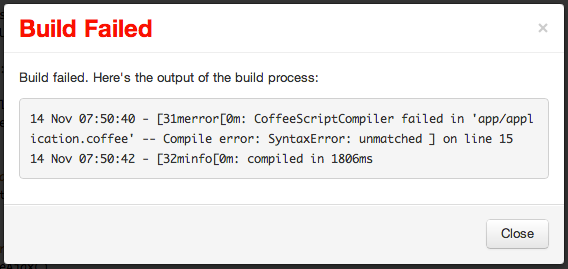
\includegraphics{figures/tutorial-error.png}
\caption{La ventana modal que se muestra al ocurrir un error de
ensamblado. \label{figures:tutorial-error}}
\end{figure}

\subsection{Archivado del Proyecto}

Una vez que el proyecto se encuentre finalizado o listo para ser subido
a un servidor, se deberá ``archivar''. Esta opción ensambla el proyecto,
con la diferencia de además minificar los archivos Javascript y CSS
generados, efectivamente optimizándolos para producción. Al presionar
esta opción, que puede verse en la Figura
\ref{figures:tutorial-contextual}, el servidor ensambla y comprime el
proyecto en un archivo ZIP, que luego comienza a descargarse.

\subsection{Otras Características}

Existen algunas características extra disponibles para el desarrollador,
que no se discutieron en detalle en el proceso de construcción.

El usuario tiene la posibilidad de reordenar la lista de archivos
abiertos, simplemente arrastrándolos. Esta característica se une a los
atajos de teclado que permiten cambiar entre archivos abiertos,
presionando las teclas \texttt{CTRL+NÚMERO} donde \texttt{NÚMERO} es un
número entre 1 y 9.

Además, para cerrar un archivo, es posible presionar \texttt{CTRL+W}.

\clearpage
\newpage

\chapter{Conclusiones}

\label{section:conclusion}

A continuación se presentarán conclusiones del presente trabajo, con
respecto a la solución lograda y conclusiones para trabajo futuro.

\section{Sobre la Solución}

Después de algunos experimentos iniciales de prototipado de interfaces,
se estimó que desarrollar aplicaciones usando Switch IDE podría ahorrar
aproximadamente un 30\% del tiempo invertido en el prototipado de
interfaces.

Se cree que la solución que se presenta en este documento podría ayudar
a disminuir los tiempos de desarrollo de aplicaciones web, en cierta
medida facilitando la tarea que más tiempo consume. Usando Switch IDE,
se podría facilitar gran parte de esta tarea proveyendo al desarrollador
con widgets utilizados comúnmente en el desarrollo de aplicaciones, como
botones, formularios, tablas, entre otras.

\section{Trabajo Futuro}

\label{section:future-work}

Una característica que podría disminuir los tiempos de prototipado sería
la de poder ``unir'' elementos con acciones en el editor de vistas. Por
ejemplo, al agregar un botón, el desarrollador podría conectarlo con el
controlador de manera que al hacer click se ejecutara una determinada
acción. Por ejemplo, en Xcode {[}7{]} es posible presionar \texttt{CTRL}
y arrastrar el componente hacia el código, generéndose una acción que se
ejecutaría al presionar el componente (ver Figura
\ref{figure:xcode-ctrl-drag}).

\begin{figure}[htbp]
\centering
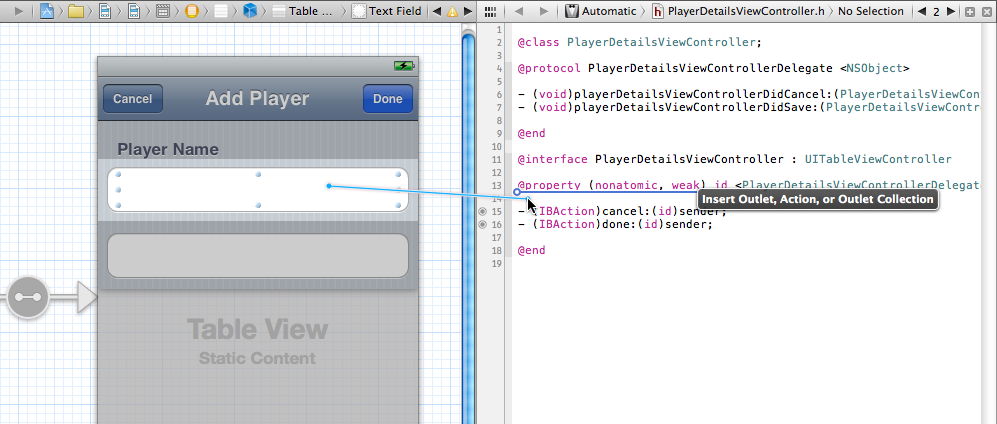
\includegraphics{figures/xcode-ctrl-drag.png}
\caption{En Xcode, al presionar la tecla \texttt{CTRL} y arrastrar un
widget, es posible crear métodos directamente.
\label{figure:xcode-ctrl-drag}}
\end{figure}

Una de las características que podría facilitar el trabajo de un
desarrollador con esta herramienta es control de versiones con Git.
Agregar esta característica no sería trivial, pero tampoco sería
extremadamente difícil dado que existen librerías que lo facilitarían.
Agregar esta funcionalidad permitiría a los desarrolladores mantener su
código versionado y además permitiría la colaboración, por medio de
repositorios compartidos. Agregar esta funcionalidad requeriría de
interfaces que permitan al desarrollador seleccionar archivos para
agregar al repositorio, crear nuevos ``commits'' (como se le conoce a
los estados de código en versionamiento), descargar y subir cambios a
repositorios remotos y poder ver el historial del repositorio.

Otra característica importante es la de no necesitar ensamblar el
proyecto constantemente. Brunch (el ensamblador que se utilizó en este
trabajo) permite levantar un proceso que observa cambios en los archivos
y ensambla el proyecto bajo demanda. De poseer esta característica en la
solución, el proceso de programar y probar los cambios podría tornarse
más continuo y simple. Sin embargo, esto requeriría cambiar la forma en
la que se levanta el servidor de pruebas, de manera de mantenerlo
siempre en línea.

Una adición que se cree agilizaría el trabajo en proyectos con archivos
grandes es la de no enviar el archivo completo cada vez que se guarden
cambios. Este es el comportamiento actual y, si bien no se nota para
archivos livianos, sí se sentiría al momento de guardar archivos
relativamente grandes. Una posible solución sería enviar parches, es
decir, guardar en el frontend el estado en el que se encuentra el
archivo en el servidor, y, al momento de guardar cambios, enviar sólo
las diferencias, optimizando la cantidad de información enviada. Por
ejemplo, si se tuviera un archivo con 200 líneas de código y sólo se
quisiera agregar 2 líneas con comentarios, sólo se tendría que
transmitir aproximadamente un 1\% del archivo.

En cuando a optimizaciones, si bien Javascript es un lenguaje con
recolección de basura y el desarrollador no debería preocuparse del
manejo de memoria, en Backbone es muy fácil comenzar a fugar (``leak'',
en inglés) objetos a memoria. Esto es porque la recolección de basura
sólo elimina objetos de memoria cuando ya no existen referencias a éste.
En Backbone, al haber tantos objetos dependiendo de otros y escuchando
notificaciones de otros, aun cuando se haya eliminado una vista del
documento, el objeto seguirá escuchando eventos de otros objetos y
seguirá en memoria. Siendo este trabajo un proyecto de Backbone
relativamente grande, la posibilidad de empezar a fugar objetos es alta.
Existen algunas guías para mejorar el rendimiento de aplicaciones
escritas en Backbone como la escrita por la empresa Paydirt {[}38{]},
que convendría seguir y aplicar en este proyecto y que se cree ayudarían
a mejorar su rendimiento.

En cuando a la edición de templates, en la solución propuesta no es
posible cambiar propiedades de los diferentes widgets visualmente (como
por ejemplo cambiar el color a un botón, o cambiar ciertas propiedades
de una tabla). Se propone agregar un editor de propiedades que permita
cambiar diferentes atributos de algún componente seleccionado, de manera
de evitar que el desarrollador deba editar HTML directamente.

En la misma línea, se cree que cambiar el framework que se utiliza para
el desarrollo por una conocida como Knockback {[}46{]} podría facilitar
el trabajo del desarrollador aún más al editar templates. Knockback es
una combinación de dos frameworks: Backbone (la que se utiliza
actualmente) y Knockout. Knockout es conocido por ofrecer ``bindings'',
es decir, permite agregar atributos HTML a las vistas de manera que se
actualicen automáticamente, sin necesidad de escribir código dentro de
ellas. Como por ejemplo:

\begin{Shaded}
\begin{Highlighting}[]
\KeywordTok{<p>}\NormalTok{First name: }\KeywordTok{<strong}\OtherTok{ data-bind=}\StringTok{"text: firstName"}\KeywordTok{></strong></p>}
\KeywordTok{<p>}\NormalTok{Last name: }\KeywordTok{<strong}\OtherTok{ data-bind=}\StringTok{"text: lastName"}\KeywordTok{></strong></p>}
\end{Highlighting}
\end{Shaded}

El fragmento anterior une las etiquetas
\texttt{\textless{}strong\textgreater{}} con los atributos
\texttt{firstName} y \texttt{lastName} del modelo asociado. Lo ventajoso
es que es simple HTML y además las uniones son en tiempo real, lo que
significa que cualquier cambio al modelo ocurrirá en la vista sin
requerir ningún esfuerzo extra por parte del desarrollador.

Esto podría mejorar la experiencia del desarrollador al momento de
diseñar vistas dado que no necesitaría escribir código (sólo HTML).
Además, y más importante, esto permitiría mejorar el editor de
interfaces de manera de que el usuario agregue ``bindings'' visualmente,
como por ejemplo con menús contextuales, sin editar el código fuente de
la vista.

Agregar este framework podría significar un esfuerzo mayor, aunque
Brunch facilita esta tarea permitiendo crear ``esqueletos'' para
proyectos con este framework. Exportar proyectos ya existentes no sería
trivial, pero tampoco sería muy complejo, dado que Knockback simplemente
combina ambos frameworks.

\clearpage
\newpage

\chapter{Referencias}

{[}1{]} Open Source Initiative, ``MIT License'' Disponible:
\href{http://opensource.org/licenses/MIT}{http://opensource.org/licenses/MIT}.
Última Revisión: 18/11/2012.

{[}2{]} Steve Burbeck, ``Applications Programming in Smalltalk-80(TM):
How to use Model-View-Controller (MVC)'' Disponible:
\href{http://st-www.cs.illinois.edu/users/smarch/st-docs/mvc.html}{http://st-www.cs.illinois.edu/users/smarch/st-docs/mvc.html}.
Última Revisión: 09/07/2012.

{[}3{]} Mike Potel, ``MVP: Model-View-Presenter. The Taligent
Programming Model for C++ and Java'' Disponible:
\href{http://www.wildcrest.com/Potel/Portfolio/mvp.pdf}{http://www.wildcrest.com/Potel/Portfolio/mvp.pdf}.
Última Revisión: 09/07/2012.

{[}4{]} DocumentCloud, ``Backbone'' Disponible:
\href{http://backbonejs.org}{http://backbonejs.org}. Última Revisión:
09/07/2012.

{[}5{]} Backbone, ``Projects and Companies using Backbone'' Disponible:
\href{https://github.com/documentcloud/backbone/wiki/Projects-and-Companies-using-Backbone}{https://github.com/documentcloud/backbone/wiki/Projects-and-Companies-using-Backbone}.
Última Revisión: 09/07/2012.

{[}6{]} Cappuccino Project, ``Cappuccino Framework'' Disponible:
\href{http://www.cappuccino-project.org/}{http://www.cappuccino-project.org/}.
Última Revisión: 09/07/2012.

{[}7{]} Apple Inc., ``Xcode'' Disponible:
\href{https://developer.apple.com/xcode/}{https://developer.apple.com/xcode/}.
Última Revisión: 09/07/2012.

{[}8{]} Sencha Inc., ``Ext JS'' Disponible:
\href{http://www.sencha.com/products/extjs/}{http://www.sencha.com/products/extjs/}.
Última Revisión: 09/07/2012.

{[}9{]} Sencha Inc., ``Ext JS Releases'' Disponible:
\href{http://www.sencha.com/products/releases/}{http://www.sencha.com/products/releases/}.
Última Revisión: 09/07/2012.

{[}10{]} Sencha Inc., ``Buy Ext JS 4 Licenses and Support'' Disponible:
\href{http://www.sencha.com/store/extjs/}{http://www.sencha.com/store/extjs/}.
Última Revisión: 09/07/2012.

{[}11{]} Sencha Inc., ``Sencha Architect'' Disponible:
\href{http://www.sencha.com/products/architect/}{http://www.sencha.com/products/architect/}.
Última Revisión: 09/07/2012.

{[}12{]} Sencha Inc., ``Buy Sencha Architect'' Disponible:
\href{http://www.sencha.com/store/architect/}{http://www.sencha.com/store/architect/}.
Última Revisión: 09/07/2012.

{[}13{]} Divshot, ``Divshot'' Disponible:
\href{http://www.divshot.com}{http://www.divshot.com}. Última Revisión:
09/07/2012.

{[}14{]} Twitter, ``Twitter Bootstrap'' Disponible:
\href{http://getbootstrap.com}{http://getbootstrap.com}. Última
Revisión: 09/07/2012.

{[}15{]} Ian Hickson (editor), ``HTML5 Specification'' Disponible:
\href{http://www.w3.org/TR/2011/WD-html5-20110525/}{http://www.w3.org/TR/2011/WD-html5-20110525/}.
Última Revisión: 09/07/2012.

{[}16{]} eXo Platform SAS, ``eXo Cloud IDE'' Disponible:
\href{http://cloud-ide.com}{http://cloud-ide.com}. Última Revisión:
09/07/2012.

{[}17{]} Git Project, ``Git'' Disponible:
\href{http://git-scm.com}{http://git-scm.com}. Última Revisión:
09/07/2012.

{[}18{]} Twitter Inc., ``Twitter Bootstrap'' Disponible:
\href{https://github.com/twitter/bootstrap}{https://github.com/twitter/bootstrap}.
Última Revisión: 18/11/2012.

{[}19{]} GitHub Inc., ``Popular Starred Repositories'' Disponible:
\href{https://github.com/popular/starred}{https://github.com/popular/starred}.
Última Revisión: 18/11/2012.

{[}20{]} TIOBE, ``TIOBE Programming Community Index for November 2012''
Disponible:
\href{http://www.tiobe.com/index.php/content/paperinfo/tpci/index.html}{http://www.tiobe.com/index.php/content/paperinfo/tpci/index.html}.
Última Revisión: 18/11/2012.

{[}21{]} EllisLab, ``CodeIgniter'' Disponible:
\href{http://codeigniter.com}{http://codeigniter.com}. Última Revisión:
18/11/2012.

{[}22{]} Play, ``Play Framework'' Disponible:
\href{http://www.playframework.org}{http://www.playframework.org}.
Última Revisión: 18/11/2012.

{[}23{]} Django Software Foundation, ``Django Framework'' Disponible:
\href{https://www.djangoproject.com}{https://www.djangoproject.com}.
Última Revisión: 18/11/2012.

{[}24{]} Ruby on Rails, ``Ruby on Rails Framework'' Disponible:
\href{http://rubyonrails.org}{http://rubyonrails.org}. Última Revisión:
18/11/2012.

{[}25{]} Tom Preston-Werner, ``Grit'' Disponible:
\href{https://github.com/mojombo/grit}{https://github.com/mojombo/grit}.
Última Revisión: 18/11/2012.

{[}26{]} Hot Frameworks, ``Ruby Framework Rankings'' Disponible:
\href{http://hotframeworks.com/languages/ruby}{http://hotframeworks.com/languages/ruby}.
Última Revisión: 18/11/2012.

{[}27{]} ORACLE, ``MySQL'' Disponible:
\href{http://www.mysql.com}{http://www.mysql.com}. Última Revisión:
18/11/2012.

{[}28{]} 10gen Inc., ``MongoDB'' Disponible:
\href{http://www.mongodb.org}{http://www.mongodb.org}. Última Revisión:
18/11/2012.

{[}29{]} ORACLE, ``MySQL Market Share'' Disponible:
\href{http://www.mysql.com/why-mysql/marketshare}{http://www.mysql.com/why-mysql/marketshare}.
Última Revisión: 18/11/2012.

{[}30{]} D. Crockford, ``The application/json Media Type for JavaScript
Object Notation (JSON)'' Disponible:
\href{http://www.ietf.org/rfc/rfc4627.txt?number=4627}{http://www.ietf.org/rfc/rfc4627.txt?number=4627}.
Última Revisión: 18/11/2012.

{[}31{]} 10gen Inc., ``GridFS'' Disponible:
\href{http://www.mongodb.org/display/DOCS/GridFS}{http://www.mongodb.org/display/DOCS/GridFS}.
Última Revisión: 18/11/2012.

{[}32{]} Ruby on Rails, ``Active Record -- Object-relational mapping put
on rails'' Disponible:
\href{https://github.com/rails/rails/tree/master/activerecord}{https://github.com/rails/rails/tree/master/activerecord}.
Última Revisión: 18/11/2012.

{[}33{]} Durran Jordan, ``Mongoid'' Disponible:
\href{http://mongoid.org}{http://mongoid.org}. Última Revisión:
18/11/2012.

{[}34{]} Nik Graf, Thomas Schranz, Andreas Gesrtmayr Paul Miller,
``Brunch'' Disponible: \href{http://brunch.io}{http://brunch.io}. Última
Revisión: 18/11/2012.

{[}35{]} Knockout, ``Knockout'' Disponible:
\href{http://knockoutjs.com}{http://knockoutjs.com}. Última Revisión:
18/11/2012.

{[}36{]} Jeremy Ashkenas, ``CoffeeScript'' Disponible:
\href{http://coffeescript.org}{http://coffeescript.org}. Última
Revisión: 18/11/2012.

{[}37{]} Tilde Inc., ``Ember.js'' Disponible:
\href{http://emberjs.com}{http://emberjs.com}. Última Revisión:
18/11/2012.

{[}38{]} Nicholas Firth-McCoy, ``Backbone.js in Practice: Part I --
Preventing Memory Leaks'' Disponible:
\href{https://paydirtapp.com/blog/backbone-in-practice-memory-management-and-event-bindings/}{https://paydirtapp.com/blog/backbone-in-practice-memory-management-and-event-bindings/}.
Última Revisión: 18/11/2012.

{[}39{]} Microsoft, ``TypeScript'' Disponible:
\href{http://www.typescriptlang.org/}{http://www.typescriptlang.org/}.
Última Revisión: 18/11/2012.

{[}40{]} Roy Fielding, ``Representational State Transfer (REST)''
Disponible:
\href{http://www.ics.uci.edu/~fielding/pubs/dissertation/rest\_arch\_style.htm}{http://www.ics.uci.edu/\textasciitilde{}fielding/pubs/dissertation/rest\_arch\_style.htm}.
Última Revisión: 18/11/2012.

{[}41{]} Terence Lee, André Arko, ``Bundler'' Disponible:
\href{http://gembundler.com}{http://gembundler.com}. Última Revisión:
18/11/2012.

{[}42{]} Marijn Haverbeke, ``CodeMirror'' Disponible:
\href{http://codemirror.net}{http://codemirror.net}. Última Revisión:
18/11/2012.

{[}43{]} Nodejitsu, ``Forever'' Disponible:
\href{https://github.com/nodejitsu/forever}{https://github.com/nodejitsu/forever}.
Última Revisión: 18/11/2012.

{[}44{]} Craig Campbell, ``Mousetrap'' Disponible:
\href{http://craig.is/killing/mice}{http://craig.is/killing/mice}.
Última Revisión: 18/11/2012.

{[}45{]} The jQuery Foundation, ``jQuery UI'' Disponible:
\href{http://jqueryui.com}{http://jqueryui.com}. Última Revisión:
18/11/2012.

{[}46{]} Kevin Malakoff, ``Knockback'' Disponible:
\href{http://kmalakoff.github.com/knockback}{http://kmalakoff.github.com/knockback}.
Última Revisión: 18/11/2012.

\end{document}
